\documentclass{beamer}

\mode<presentation>

{
\usetheme{Rochester}
\setbeamercovered{transparent}
}

\usecolortheme{wolverine}

\usepackage{amsmath}
\usepackage{amsfonts}
\usepackage{amssymb}
\usepackage[english]{babel}
\usepackage{graphicx}
\usepackage[utf8]{inputenc}
\usepackage[T1]{fontenc}
%\usepackage[natbib=true, style=thesis, url=false, doi=false, firstinits=true, defernumbers=true, bibstyle=numeric, title=false, sorting=ydnt, citestyle=authoryear-comp, isbn=false]{biblatex}
\usepackage{lmodern}
\usepackage{hyperref}
\usepackage{lscape}
\usepackage{multirow}
\usepackage[parfill]{parskip}
\usepackage{makeidx}
%\usepackage{times}
%\bibliography{library}
\usepackage{wrapfig}
\usepackage{pgf}
\usepackage{fancybox}
\usepackage{multimedia}
%\usepackage[]{movie15}

\newcommand{\obs}{\mathrm{obs}}
\newcommand{\pred}{\mathrm{pred}}
\newcommand{\eff}{\mathrm{eff}}
\newcommand{\intt}{\mathrm{int}}
\newcommand{\LMC}{\mathrm{LMC}}
\newcommand{\MW}{\mathrm{MW}}
\newcommand{\Cepheid}{\mathrm{Cepheid}}
\newcommand{\Anchors}{\mathrm{Anchors}}
\newcommand{\SNe}{\mathrm{SNe\,Ia}}
\newcommand{\km}{\mathrm{km}}
\newcommand{\second}{\mathrm{s}}
\newcommand{\Mpc}{\mathrm{Mpc}}
\newcommand{\MAnd}{\mathrm{M31}}
\newcommand{\NGC}{\mathrm{NGC4258}}
%\def\be{\begin{equation}}
%\def\ee{\end{equation}}
%\def\bea{\begin{eqnarray}}
%\def\eea{\end{eqnarray}}


\author[Wilmar Alberto Cardona Castro]{Wilmar Alberto Cardona Castro}
%\institute[]{University of Geneva}
%\date{18th June, 2012}

\title[Cosmological constraints: anisotropic dark energy, the Hubble constant, and the neutrino mass]{Cosmological constraints: anisotropic dark energy, the Hubble constant, and the neutrino mass}
\subject{Cosmology}


\beamerdefaultoverlayspecification{<+->}
\setbeamertemplate{footline}[frame number]
\begin{document}

%\begin{frame}{\textit{Planck} (and some external data sets) constraints}
%\begin{columns}
%\begin{column}{0.45\textwidth}
%\centering
%\only<1-3>{TT+TE+EE+lowP+BAO
%\includegraphics[scale=0.65]{./Neff-H0.pdf}
%} 
%\only<4-7>{TT+lowP+BAO+JLA
%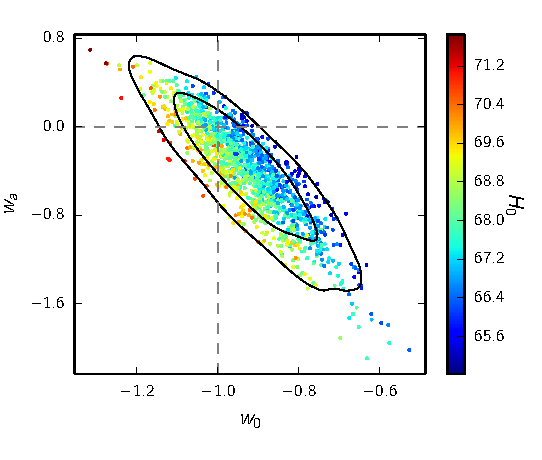
\includegraphics[scale=0.65]{./w-H0.pdf}
%}
%\end{column}
%\begin{column}{0.45\textwidth}
%\centering
%\only<1-3>{TT+lowP+lensing
%\includegraphics[scale=0.65]{./mnu-H0.pdf}} 
%\only<5-7>{Direct vs. Indirect 
%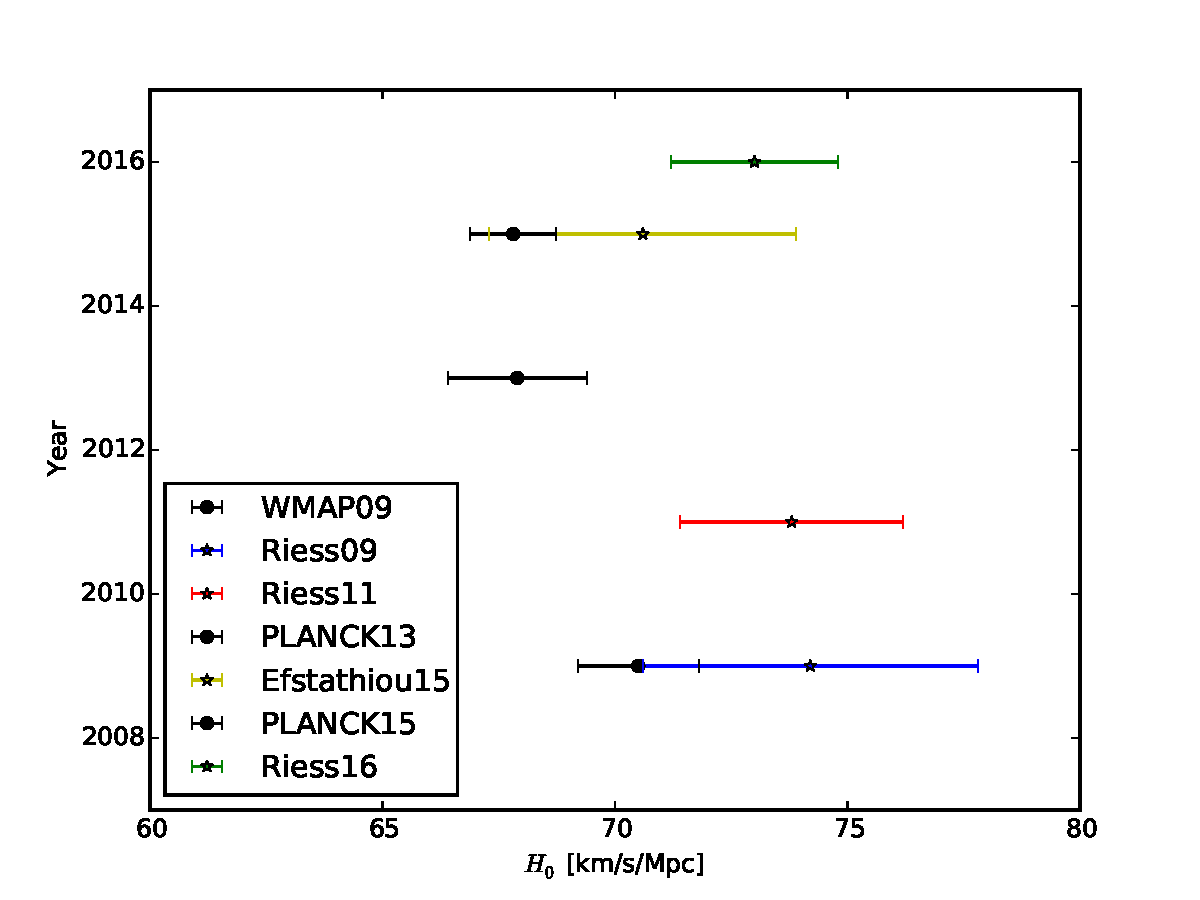
\includegraphics[scale=0.3]{./H0_values.pdf}}
%%\only<4>{Inpainted NILC 
%%\includegraphics[scale=0.2]{../../../../../projects/B/ksv-maps/planck-nside/nilc/192c/inpainted/vmap.pdf}}
%\end{column}
%\end{columns}
%\begin{center}
%\only<6>{Theoretical attempts ?}
%\only<7>{Issues in the statistical analysis ?}
%\end{center}

%A figure showing degeneracies (e.g, $w,\, m_\nu$).
%A figure comparing $H_0$ from direct measurements and from WMAP and PLANCK: WMAP9, R09, R11, PLANCK13, E15, PLANCK15. Discuss differences between R09 and R11, between R11 and E15 (rejection algorithm, new data for NGC4258), direct and derived $H_0$. Mention failed theoretical attempts to explain discrepancy by Ruth and Iggy.  
%\end{frame}

\begin{frame}
\begin{figure}[hbtp]
\centering
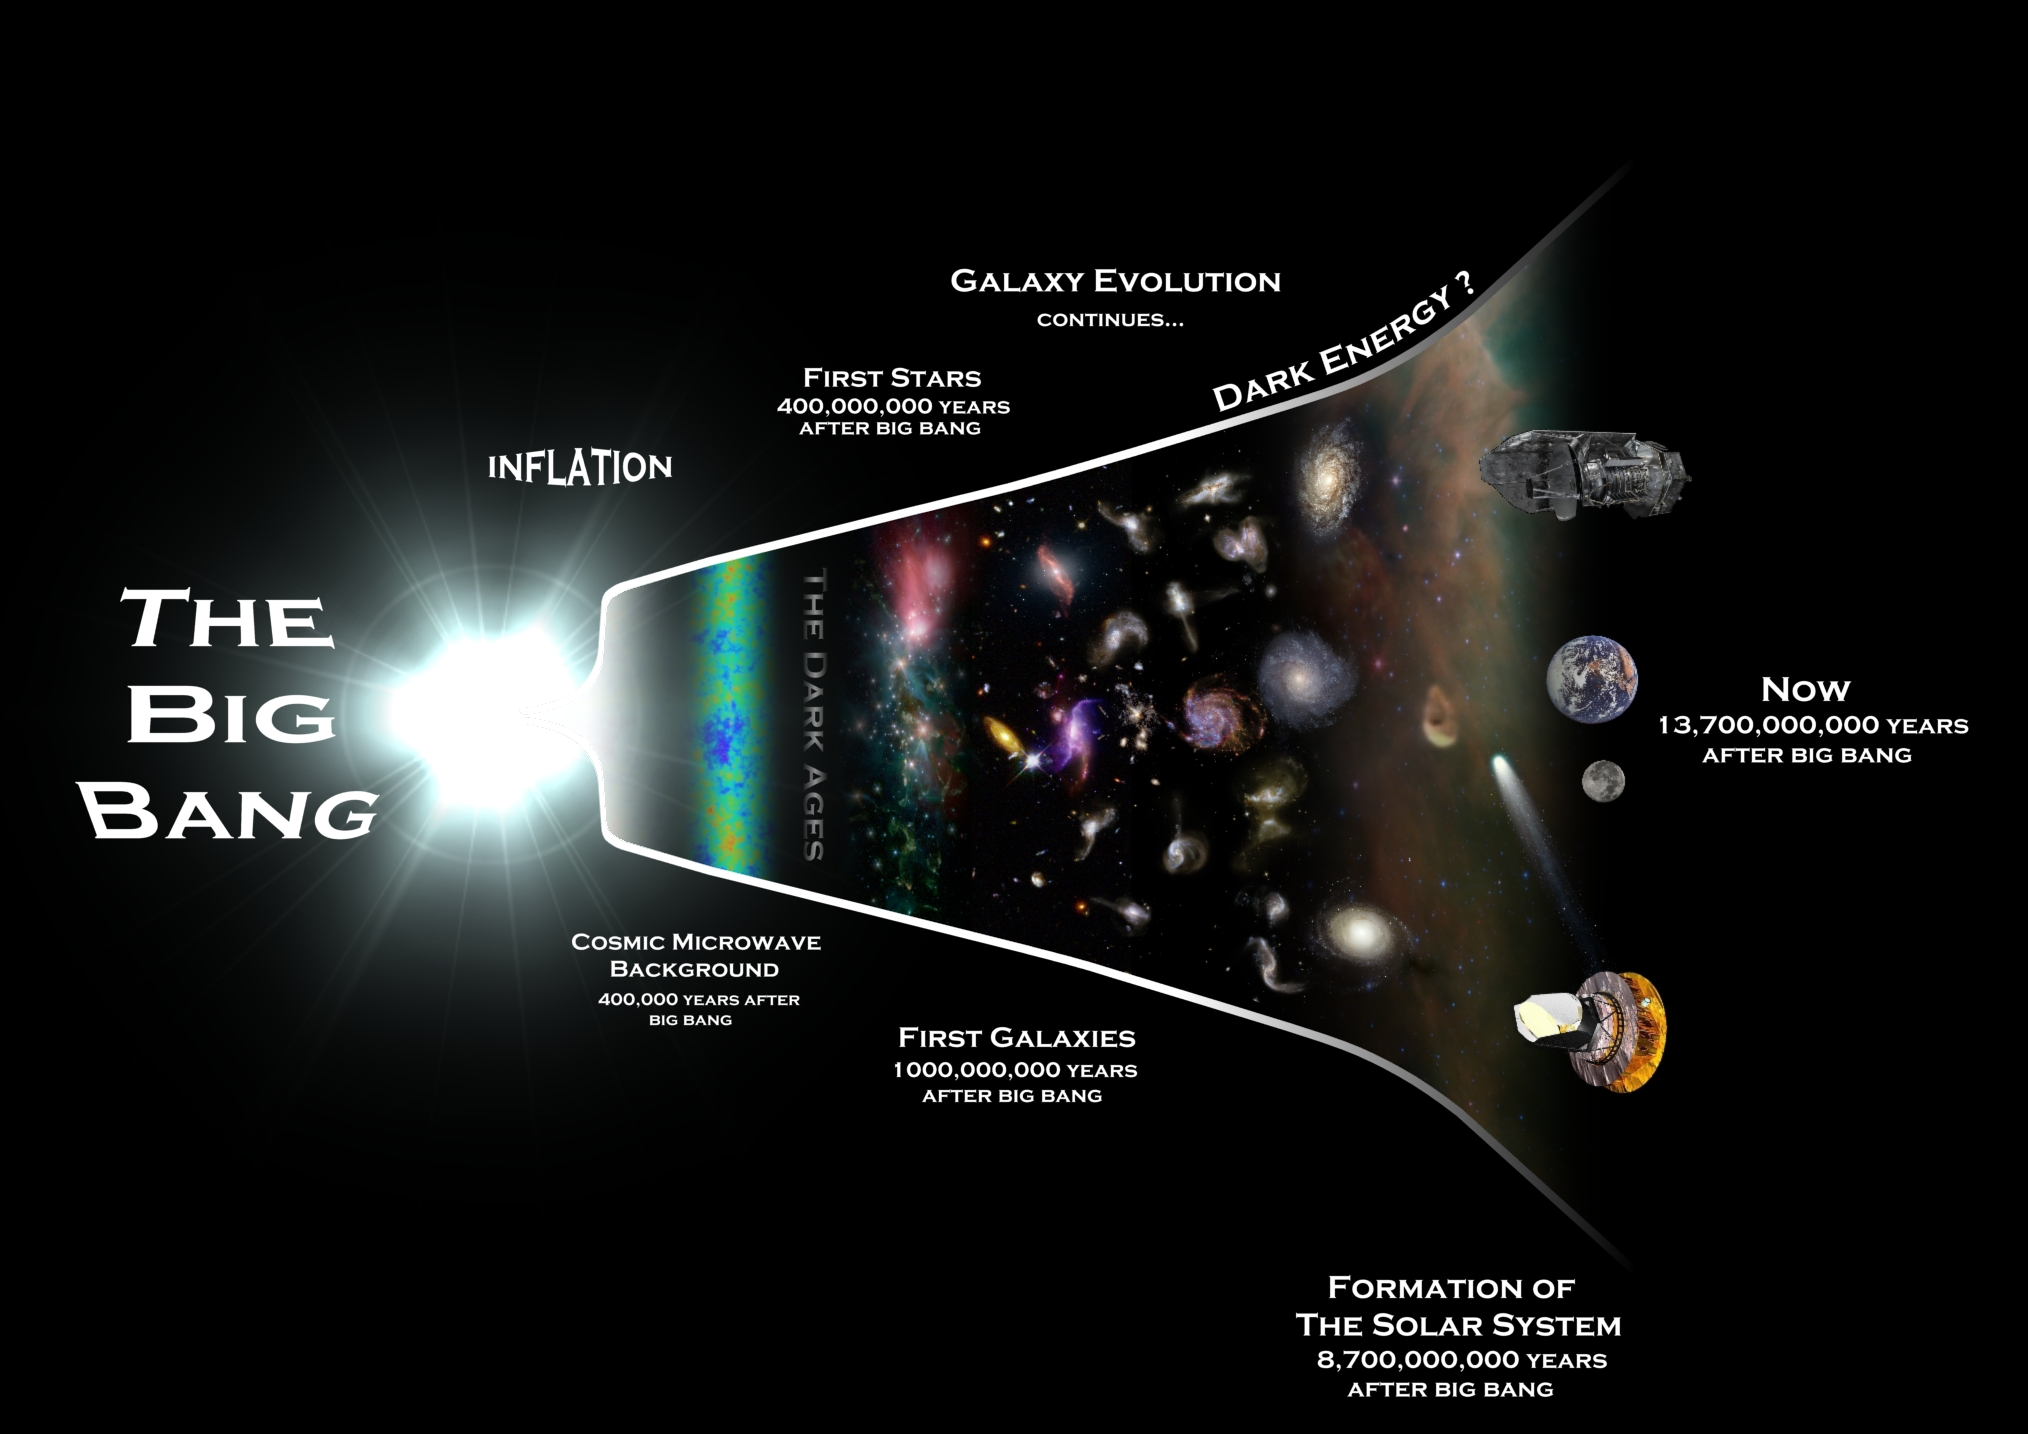
\includegraphics[width=\textwidth]{../figures/Timeline_portrait.jpg}
\end{figure}

\end{frame}

\begin{frame}
  \titlepage
\end{frame}

\begin{frame}{Contents}
  \tableofcontents
\end{frame}

\section{Brief introduction: the concordance model of cosmology}

\begin{frame}{Brief introduction: the concordance model of cosmology}{The expanding universe}
\begin{itemize}
\item Cosmological principle
\item No charge asymmetry
\item General relativity
\item Solutions for Einstein's field equations satisfying the cosmological principle
\item The universe is expanding...
\item also speeding up!
\item Matter described by standard model of particle physics is not enough to match observations
\end{itemize}
\end{frame}

\begin{frame}{Brief introduction: the concordance model of cosmology}{inflation + $\Lambda$CDM}
\begin{itemize}
\item Need Dark Matter and Dark Energy to fit the accelerating expansion
\item Universe looks flat and is not completely homogeneous
\item Inflationary epoch sets adequate initial conditions for the standard model
\item So, what is DM and what is driving the accelerating expansion ? and what mechanism produced an inflationary period in the early universe ?
\item Several possible answers 
\end{itemize}
\end{frame}

\begin{frame}{Brief introduction: the concordance model of cosmology}{Vanilla model of cosmology lacks in fundamental grounds}
\begin{itemize}
\item DM not directly observed. Neutrinos are only known candidate
\item QFT cannot explain tiny observed value of the vacuum energy
\item Then ?
\item Alternatives to explain accelerating expansion: evolving scalar fields, modify GR 
\item Degeneracy of models to explain the late-time acceleration... but also degeneracy of models to describe the very early universe (inflationary models)
\item This thesis basically focuses on cosmological constraints: is it possible to break model degeneracies ? reliable constraints ? What effects are important ? Objective constraints  
\end{itemize}
\end{frame}

\begin{frame}{Brief introduction: the concordance model of cosmology}

\end{frame}

\begin{frame}{Brief introduction: the concordance model of cosmology}

\end{frame}

\begin{frame}{Brief introduction: the concordance model of cosmology}

\end{frame}

\begin{frame}{Brief introduction: the concordance model of cosmology}

\end{frame}

\begin{frame}{Brief introduction: the concordance model of cosmology}

\end{frame}

\begin{frame}{Brief introduction: the concordance model of cosmology}

\end{frame}

\begin{frame}{Brief introduction: the concordance model of cosmology}

\end{frame}

\section{Project 1: testing a fundamental assumption of the standard model of cosmology}

\begin{frame}{Project 1: testing a fundamental assumption of the standard model of cosmology}{Why do we care about the cosmological principle ?}
\begin{itemize}
\item Statistical isotropy is fundamental in the concordance model
\item Studying statistical properties of CMB anisotropies we examine assumptions of the standard model
\item CMB anisotropies... isotropic and Gaussian distributed ? 
\item Anomalies have been found by WMAP, Planck and other groups (e.g., lack of power on large angular scales, alignment of low order multipoles, north-south asymmetry in power spectra, the so-called cold spot)
\item Unaccounted systematics, non-subtracted foreground contamination, cosmological origin ?
\item WMAP and Planck are two independent experiments... unaccounted systematics seems unlikely
\item Then, anomalies due to unresolved foreground or cosmological origin ?   
\end{itemize}
\end{frame}

\begin{frame}{Project 1: testing a fundamental assumption of the standard model of cosmology}{How do we test Gaussianity and isotropy of the CMB anisotropies ?}
\begin{itemize}
\item Utilise the VSK method
\item Works in real space: localising possible non-subtracted foregrounds, may provide angular scale of possible deviations of Gaussianity and isotropy
\item Remove both monopole and dipole from CMB maps
\item Superimpose on the CMB map a Healpix grid with much lower resolution
\item For each new pixel, compute sample variance, sample skewness, and sample kurtosis 
\item The result is three functions on the sphere: a map of sample variance, a map of sample skewness, and a map of sample kurtosis
\item Repeat the above procedure for data and Gaussian isotropic simulations
\item Compute zero mean maps (variance, skewness, and kurtosis)
\item Compute angular power spectrum of the resulting maps
\item Quantify the degree of agreement data and Gaussian simulations through a $\chi^2$ test for each kind of map 
\end{itemize}
\end{frame}

\begin{frame}{Project 1: testing a fundamental assumption of the standard model of cosmology}{Applying the VSK method to Planck data}
\begin{itemize}
\item 2013 Planck release 
\item Component separation: Commander-ruler, NILC, SEVEM, SMICA
\item Inpainted CMB maps: SMICA and NILC
\item Masks: U73, VALMASK, INPMASK
\item Different resolution of CMB maps and VSK method
\item 2000 Gaussian, isotropic CMB maps
\end{itemize}
\end{frame}

\begin{frame}{Project 1: testing a fundamental assumption of the standard model of cosmology}{Results}
\begin{itemize}
\item Example of V-map
\item Example of angular power spectrum
\item Example of $\chi^2$ test
\item Table summarising results for inpainted maps
\item Table summarising dependence on CMB map resolution and VSK method resolution
\item Table dependence on the sky fraction
\item Figure comparison component separation
\end{itemize}
\end{frame}

\begin{frame}{Project 1: testing a fundamental assumption of the standard model of cosmology}

\end{frame}

\section{Project 2: constraints on anisotropic dark energy}

\begin{frame}{Project 2: constraints on anisotropic dark energy}{Why do we care about anisotropic dark energy ?}
\begin{itemize}
\item No clear explanation for the accelerating expansion of the universe
\item Two leading approaches: an unobserved fluid dubbed dark energy (DE) or modify Einstein's theory of gravity on large scales
\item A general fluid can be characterised by equation of state, sound speed, and anisotropic stress
\item Literature has focused on the background evolution, but what about DE perturbations ?  
\item Anisotropic stress is a key feature: it allows to distinguish standard DE model ($\Pi_{\rm de} = 0$) from modified gravity models ($\Pi_{\rm de}\neq 0$)
\end{itemize}
\end{frame}

\begin{frame}{Project 2: constraints on anisotropic dark energy}{How do we constrain anisotropic stress ?}
\begin{itemize}
\item Adopt a phenomenological approach: a DE model including a range of approaches (e.g., )
\item Find approximate solutions for DE perturbations
\item Implement the model in CAMB and do MCMC with COSMOMC 
\item Data from Planck, BAO, supernovae, but exclude $P(k)$ and $H_0$
\end{itemize}
\end{frame}

\begin{frame}{Project 2: constraints on anisotropic dark energy}{Results}
\begin{itemize}
\item The effect of anisotropic stress on CMB angular power spectrum and on the matter power spectrum
\item Constrains do not show evidence of non-zero anisotropic stress. 
\end{itemize}
\end{frame}

\begin{frame}{Project 2: constraints on anisotropic dark energy}

\end{frame}

\begin{frame}{Project 2: constraints on anisotropic dark energy}

\end{frame}

\section{Project 3: upcoming galaxy surveys, the lensing convergence and the neutrino mass}

\begin{frame}{Project 3: upcoming galaxy surveys, the lensing convergence and the neutrino mass}{Why do we care about massive neutrinos ?}
\begin{itemize}
\item Underlying physics in the standard model of cosmology remains unknown
\item Cold Dark Matter (CDM) constitutes  about $30\%$ of the energy content
\item Neutrinos are the only known dark matter candidate
\item Neutrinos are massive, but their absolute scale remains unconstrained
\end{itemize}
\end{frame}

\begin{frame}{Project 3: upcoming galaxy surveys, the lensing convergence and the neutrino mass}{How do we observe the effect of massive neutrinos ?}
\begin{itemize}
\item Signatures of massive neutrinos in observations: CMB anisotropies and galaxy distribution
\item Neutrinos change background evolution. For small neutrino masses, CMB can only provide upper limit 
\item Degeneracies degrade constraints from CMB data
\item Galaxy surveys come in to the rescue: probe low red-shift universe, break degeneracies
\item Massive neutrinos suppress clustering of galaxies at small scales, future surveys will hopefully take advantage of this
\item Upcoming surveys will probe distances comparable to the Hubble horizon: relativistic effects must be consistently included in the analysis
\end{itemize}

\end{frame}

\begin{frame}{Project 3: upcoming galaxy surveys, the lensing convergence and the neutrino mass}{Galaxy number counts angular power spectrum $C_\ell(z,z')$}
\begin{itemize}
\item $P(k,z)$ is not an observable. $C_\ell(z,z')$ is an observable
\item Galaxy number counts for a survey with limiting magnitude
\item Expand in spherical harmonics, taking into account red-shift dependence
\item Assume statistical isotropy and compute angular power spectrum 
\item In practice, divide the catalogue in red-shift bins 
\end{itemize}
\end{frame}

\begin{frame}{Project 3: upcoming galaxy surveys, the lensing convergence and the neutrino mass}{How do we estimate the importance of neglecting lensing convergence ?}
\begin{itemize}
\item Fit a model neglecting the effect to data ()
\item Fit a model neglecting the effect to data, but only use auto-correlations (close to $P(k)$ analysis)
\item Fit a model consistently including the effect 
\item Conservative treatment of non-linearities
\item Include shot-noise (galaxy distribution is not a continuous field)
\item Number counts alone 
\item Number counts and use CMB information from Planck
\end{itemize}
\end{frame}

\begin{frame}{Project 3: upcoming galaxy surveys, the lensing convergence and the neutrino mass}{Results}
\begin{itemize}
\item Triangle plot including CMB information
\item Table showing biased parameters: spurious detection of neutrino mass
\item Plot showing auto- and cross-correlations, equation showing dominant contribution
\item Lensing convergence must be included in the analysis of upcoming galaxy surveys, with appropriate magnification bias
\end{itemize}
\end{frame}

\section{Project 4: measuring the Hubble constant}

\begin{frame}{Project 4: measuring the Hubble constant}{Why do we care about a local measurement of $H_0$?}
\only<1-2>{\begin{figure}[hbtp]
\centering
\includegraphics[scale=0.55]{../figures/chapter-h0/mnu-H0.pdf}
\includegraphics[scale=0.55]{../figures/chapter-h0/Neff-H0.pdf}
\end{figure}}
\only<3-6>{\begin{figure}[hbtp]
\centering
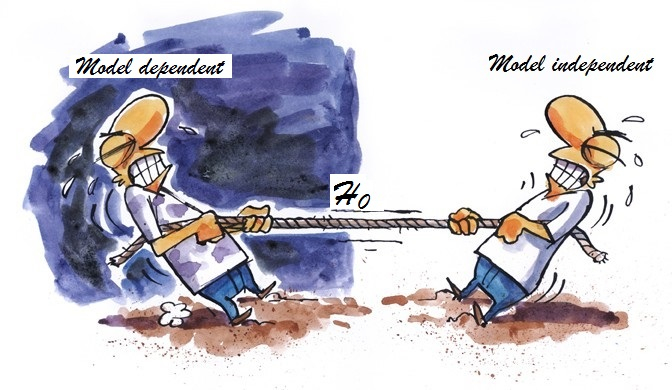
\includegraphics[scale=0.4]{../figures/chapter-h0/dependent-vs-independent.jpg}
\end{figure}}

\begin{itemize}
\only<1-2>{
\item Crucial for understanding the standard model of cosmology (i.e., it sets cosmological scales, tackle cosmological parameters and break degeneracies)
\item Inferred determinations are model dependent (e.g., properties of neutrinos, theory of gravity, nature of dark energy) and might be affected by assumed prior probability distributions}
\only<3>{
\item There is a $3.4\sigma$ tension between direct and inferred determinations of $H_0$}
\only<4>{
\item New physics (e.g., modifying assumptions in the concordance model), contributions of the local gravitational potential, unaccounted second-order corrections to the background distance-redshift relation ? }
\only<5>{
\item Issues with statistical analysis (e.g., outlier rejection algorithms, anchors choice, period cut-off and assumptions in the Leavitt law, unaccounted systematics) ?
}
\only<6>{
\item Need to confirm $3.4\sigma$ tension and prove it robust against different statistical approaches. 
}
\end{itemize}
\end{frame}

%\begin{frame}{Project 4: measuring the Hubble constant}{Why do we care about a local measurement of $H_0$?}
%\begin{itemize}
%
% 
%\end{itemize}
%
%\end{frame}

\begin{frame}{Project 4: measuring the Hubble constant}{How do we measure $H_0$?}
\only<1-4>{\begin{figure}[hbtp]
\centering
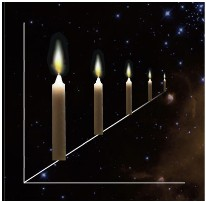
\includegraphics[scale=0.8]{../figures/chapter-h0/light-candles.jpg}
\end{figure}}
\only<8>{\begin{figure}[hbtp]
\centering
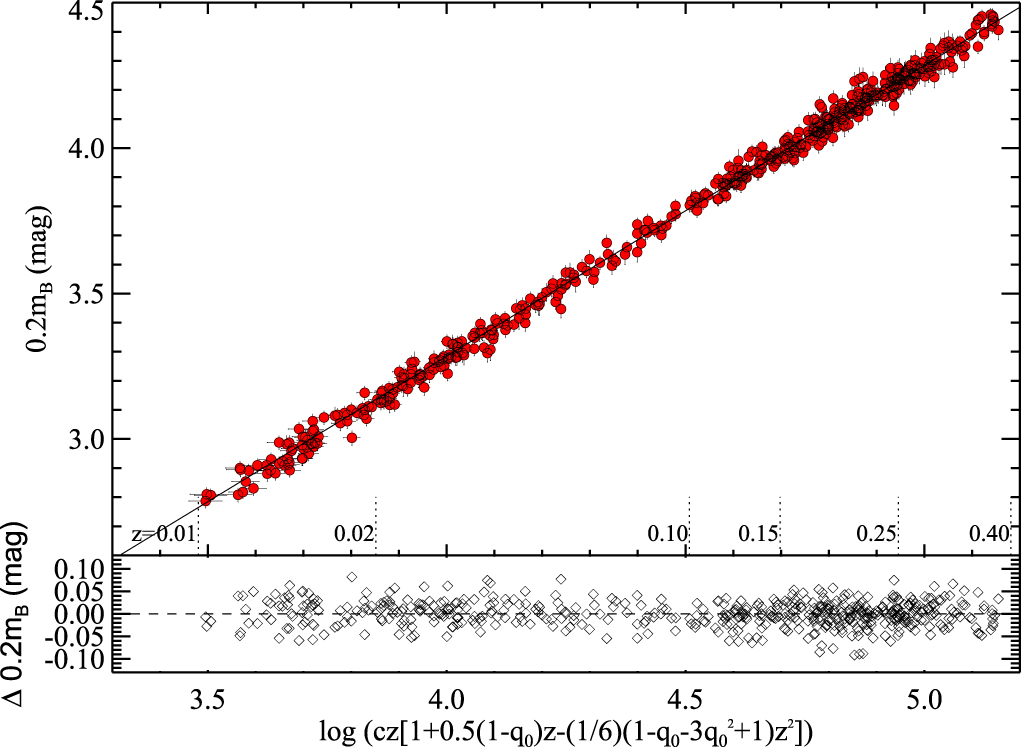
\includegraphics[scale=0.8]{../figures/chapter-h0/Hubble-diagram.jpg}
\end{figure}}

\begin{itemize}
\only<1>{
\item Estimate distances through luminosity distance
\begin{equation*}
d_L \equiv \left(\frac{L}{4\pi l} \right)^{1/2} \, \label{Eq:luminosity-distance-obs}
\end{equation*}}
\only<2-3>{
\item Define logarithmic measures of the luminosity%: absolute and apparent magnitudes
\only<2>{
\begin{equation*}\label{Eq:apparent-luminosity}
l = 10^{-2m/5}\times 2.52 \times 10^{-5}\, \mathrm{erg/ cm^2}\, \second
\end{equation*}}
\only<3>{
\begin{equation*}\label{Eq:absolute-luminosity}
L = 10^{-2M/5} \times 3.02 \times 10^{35}\, \mathrm{erg/}\second.
\end{equation*}}}
\only<4>{
\item Express luminosity distance through the distance modulus
\begin{equation*}
\mu_0 \equiv m - M = 5 \log_{10} \left(\frac{d_L}{1 \mathrm{Mpc}} \right) + 25 \,  \label{Eq:distance-modulus}
\end{equation*}}
\only<5>{
\item Assuming flat FLRW metric one can compute luminosity distance
\begin{equation*}\label{Eq:luminosity-distance-the}
d_L(z) = (1+z) c \int_0^z \frac{dz'}{H(z')} \, 
\end{equation*}}
\only<6-7>{
\item For relatively small redshift one has
\begin{equation*}\label{Eq:luminosity-distance-the-small-z}
d_L(z) \equiv \frac{cz}{H_0}  ( 1+\delta(z)) %%\approx \frac{cz}{H_0} \left\{ 1 + \frac{1}{2} [1-q_0] z - \frac{1}{6} [1-q_0 - 3 q_0^2 + j_0] z^2 + O(z^3) \right\}
\end{equation*}
\item Recalling
\begin{equation*}
\mu_0 \equiv m - M = 5 \log_{10} \left(\frac{d_L}{1 \mathrm{Mpc}} \right) + 25 \,  \label{Eq:distance-modulus}
\end{equation*}}
\only<8>{
\item Determine constant $a_X$ with Supernova type Ia ($\SNe$))
\begin{equation*}\label{Eq:av-definition}
5 \log_{10} ( c z ( 1+\delta(z) )) - m_X = 5 \log_{10} H_0 - M_X - 25 \equiv 5 a_X \, 
\end{equation*}}
\end{itemize}
\end{frame}

\begin{frame}{Project 4: measuring the Hubble constant}{How do we measure $H_0$?}
\begin{itemize}
\only<1-3>{
\item Use now simultaneously $\SNe$ and Cepheid stars
\begin{figure}
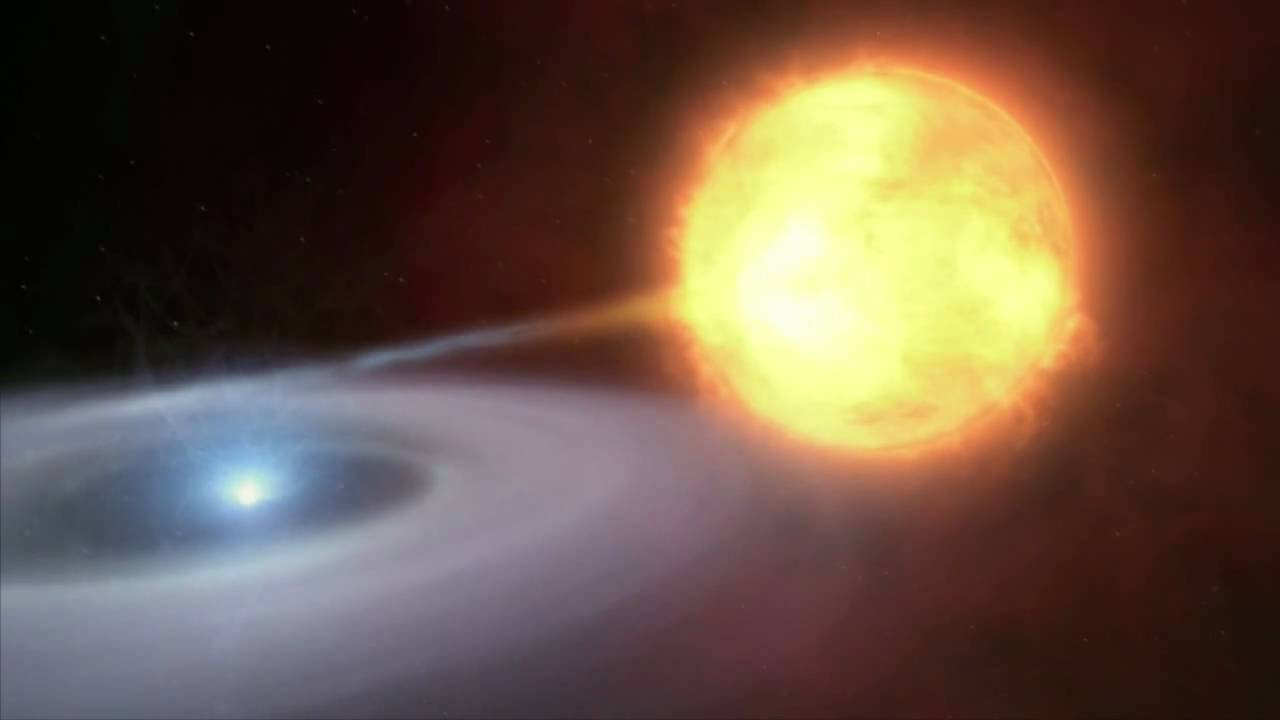
\includegraphics[scale=0.11]{../figures/chapter-h0/sntypeia.jpg}%\hspace{1mm} 
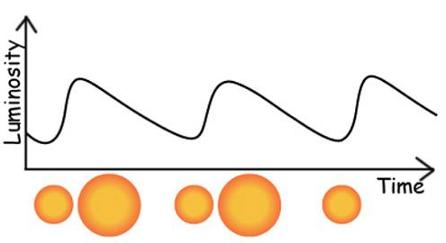
\includegraphics[scale=0.45]{../figures/chapter-h0/cepheid.jpg} 
\end{figure}}

\item $\SNe$ apparent magnitudes
\begin{equation*}
m_X^{\SNe} =  5 \log_{10} H_0 + \mu_0 - 5 a_X - 25 \, %. \label{Eq:apparent-magnitude-H0}
\end{equation*}
\item Cepheid variables apparent magnitudes 
\begin{equation*}\label{Eq:P-L-equation}
m_{Y,i,j}^{\Cepheid} = \mu_{0,i} + M_Y^{\Cepheid} + b_Y (\log P_{i,j}-1) + Z_Y \Delta \log[O/H]_{i,j}%,
\end{equation*}
\item Galaxies hosting both $\SNe$ and Cepheid stars
\item A few anchor distances: $\mu_0^\LMC$, $\mu_0^\NGC$, $\mu_0^\MAnd$, $\MW$ Cepheid stars parallaxes 
\end{itemize}
\end{frame}

\begin{frame}{Project 4: measuring the Hubble constant}{How do we measure $H_0$?}
\only<1-2>{
\begin{figure}
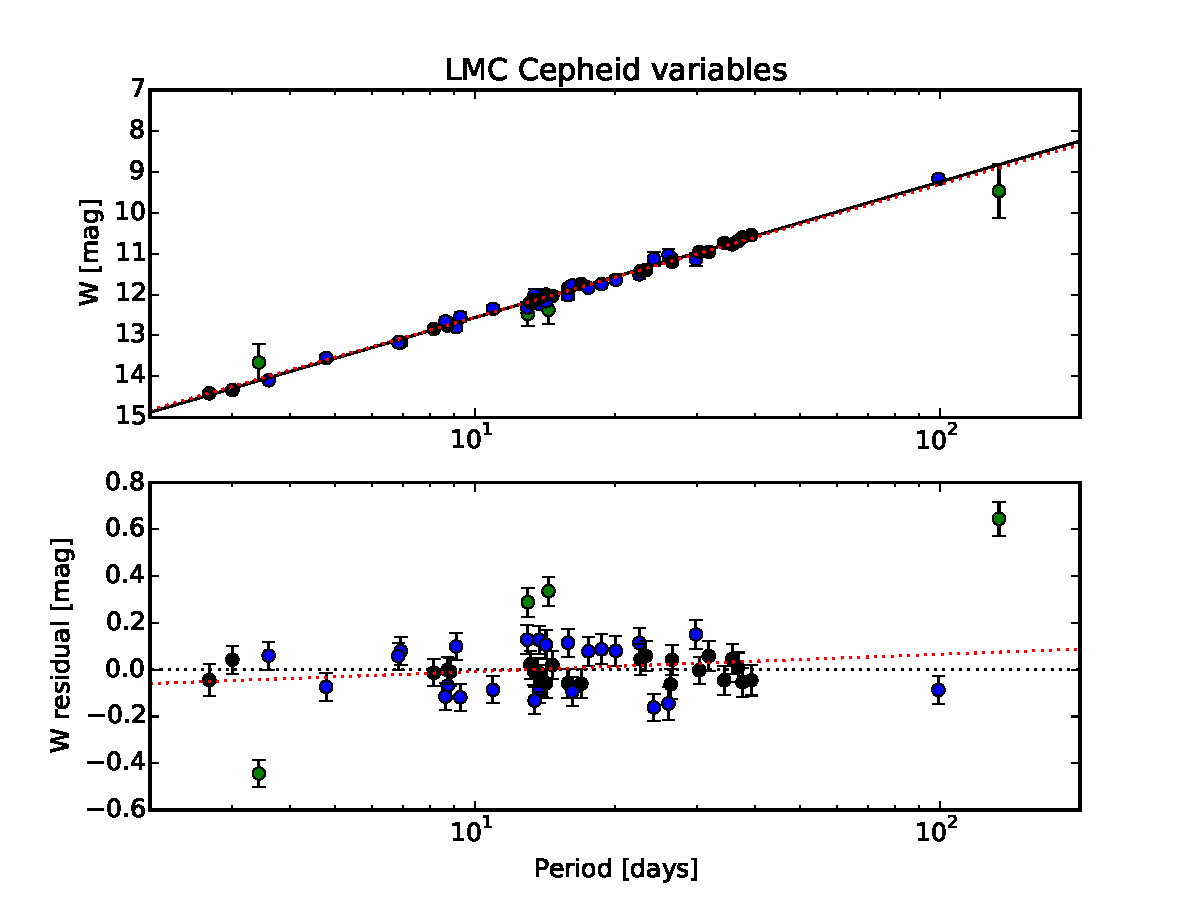
\includegraphics[scale=0.4]{../figures/chapter-h0/effective_HP_cepheids_LMC.pdf} 
\end{figure}}

\begin{itemize}
\only<1>{
\item Need to determine the best fitting parameters in the relations above, but data sets include outliers...}
\only<2>{
\item Outlier rejection algorithm or a Bayesian treatment ?}
\only<3-6>{
\item Usually assumed data points drawn from a Gaussian PDF
\begin{equation*}\label{Eq:Gaussian-likelihood}
P_G(D_i|\vec{w}) = \tilde{N}_i \, \frac{\exp(-\chi^2_i(\vec{w})/2)}{\sqrt{2\pi}}
\end{equation*}}
\only<4-6>{
\item Drop this and assume error bars can be underestimated: introduce hyper-parameters for each datum $\sigma_i \rightarrow \sigma_i/\sqrt{\alpha_i}$}
\only<5-6>{
\item Starting from usual Gaussian PDF with usual $\chi^2$, but allow error bars to become greater and take into account every possible value for the rescaling (marginalise over HPs)}
\only<6>{
\item End up with a new PDF: a Gaussian HP PDF 
\begin{equation*}
P(D_i|\vec{w}\,) = \tilde{N}_i \, \left(\frac{ \mathrm{Erf}\left( \frac{\chi_i(\vec{w})}{\sqrt{2}} \right)  -\sqrt{\frac{2}\pi} \chi_i(\vec{w}) \exp(-\chi^2_i(\vec{w})/2)}{ \chi^3_i(\vec{w})} \right)
\end{equation*}}
\only<7-8>{
\item Maximise likelihood and compute effective HPs for each datum (given the best fitting parameters)
\begin{eqnarray*}
\alpha^{\eff}_i & = 1,\quad \mathrm{if} \quad \chi^2_i\leq1
\\
\label{Eq:effective-HP-2}
\alpha^{\eff}_i & = \frac{1}{\chi^2_i},\quad \mathrm{if} \quad \chi^2_i> 1.
\end{eqnarray*}}
\only<8>{
\item Asses compatibility of data sets through normalised weights
\begin{equation*}
|| \alpha^{j} || \equiv \frac{\sum_{i=1}^{K_j} \alpha_{i,j}}{K_j},
\label{Eq:normalised-weights}
\end{equation*}} 
\end{itemize}
\end{frame}

\begin{frame}{Project 4: measuring the Hubble constant}{What data do we use ?}
\begin{itemize}
\item The R11 data set: $8$ galaxies simultaneously hosting $\SNe$ and Cepheid stars, three anchor distances ($\mu_0^\LMC$, $\mu_0^\NGC$, 13 $\MW$ Cepheid stars parallaxes)
\item The R16 data set: $19$ galaxies simultaneously hosting $\SNe$ and Cepheid stars, four anchor distances ($\mu_0^\LMC$, $\mu_0^\NGC$, $\mu_0^\MAnd$, 15 $\MW$ Cepheid stars parallaxes)
\end{itemize}
\end{frame}

\begin{frame}{Project 4: measuring the Hubble constant}{Results: the R11 data set}

\only<1>{
\begin{table}[tbp]
\centering
\begin{tabular}{@{}ccccc}
\hline
\multicolumn{5}{c}{Consistency of period-luminosity relation} \\
\hline
Fit & Galaxy & $M_W$ & $b_W$ & $\sigma_{\intt}$ \\
\hline
 c & $\LMC$ & $-5.93\,(0.07)$& $-3.31\,(0.05)$& $0.06$  \\
 
 e & $\MW$ & $-5.88\,(0.07)$ & $-3.30\,(0.26)$ & $0.02$  \\
  
 f & $\NGC$ & $-6.12\,(0.15)$&$-3.02\,(0.17)$ & $0.12$  \\

\hline
\end{tabular}
%\caption{\label{Table:fits-section-4-1} \wct{Constraints for the parameters in the period-luminosity relation. Numbers in brackets indicate the standard deviation. Fit (c) was derived using the distance modulus in Eq. \eqref{Eq:LMC-measured-distance-modulus}, fit (e) corresponds to Eq. \eqref{Eq:MW-bestfit}, and fit (f) was derived using the distance modulus in Eq. \eqref{Eq:NGC4258-measured-distance-modulus-2013}}.}
\end{table}}

\only<2>{
\begin{figure}
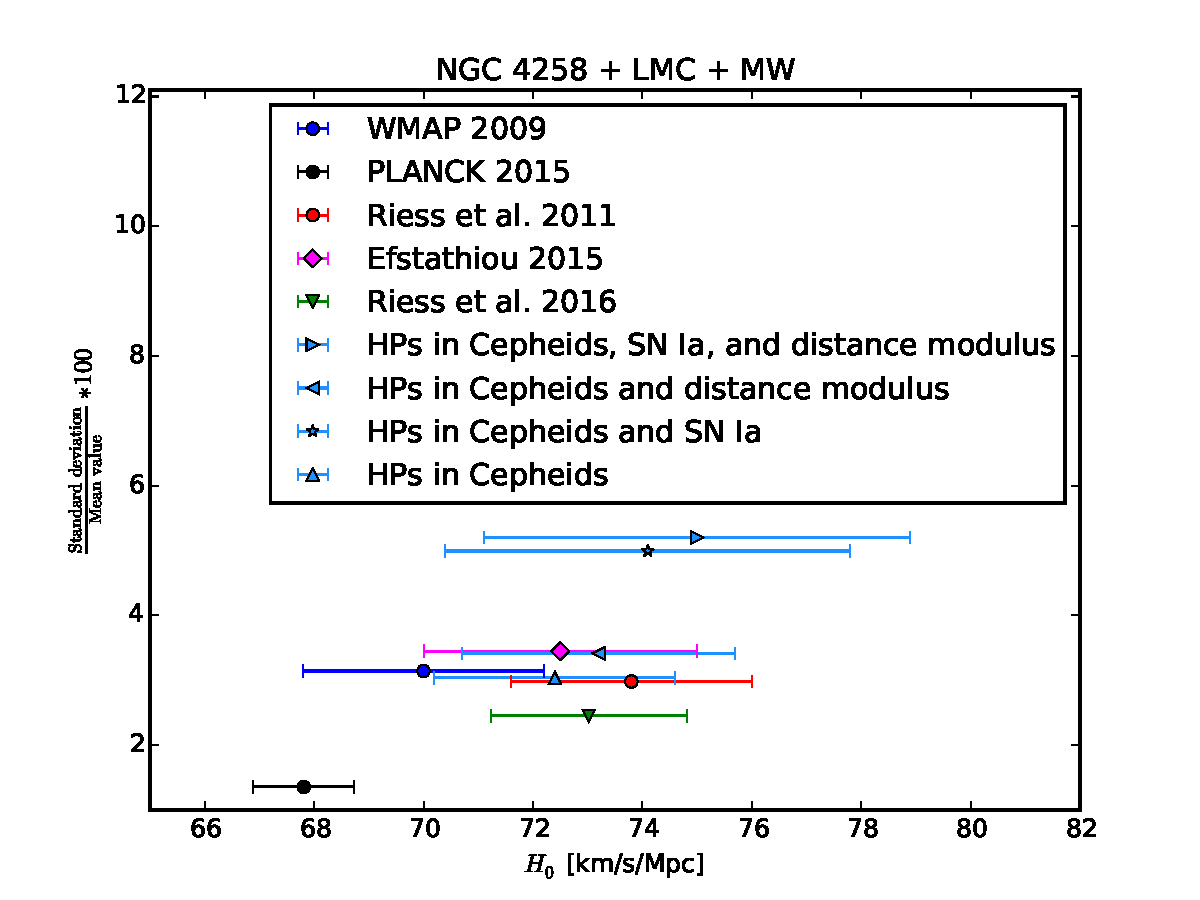
\includegraphics[scale=0.4]{../figures/chapter-h0/H0_values_three_anchors.pdf} 
\end{figure}}
\only<3>{
\begin{figure}
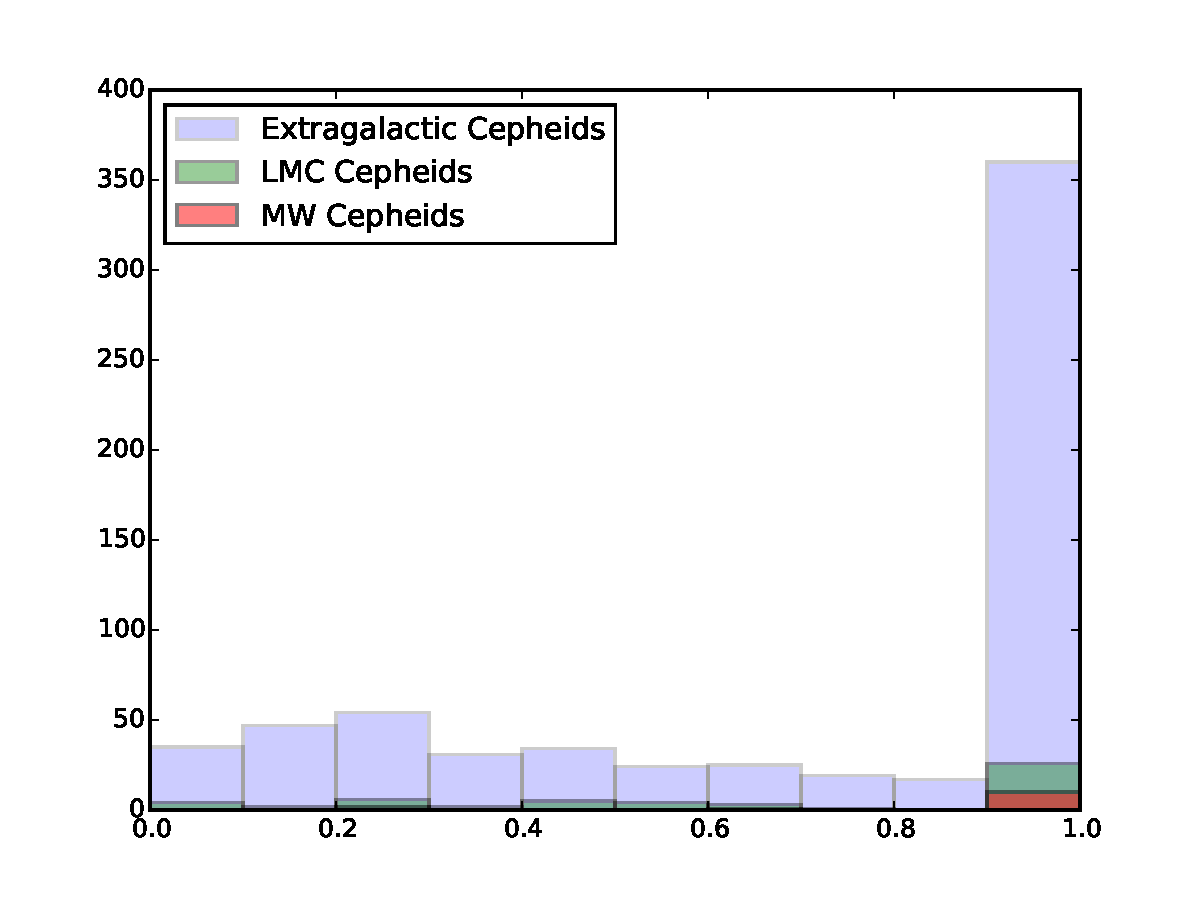
\includegraphics[scale=0.4]{../figures/chapter-h0/effective_HP_histogram.pdf} 
\end{figure}}
\only<4>{
\begin{figure}
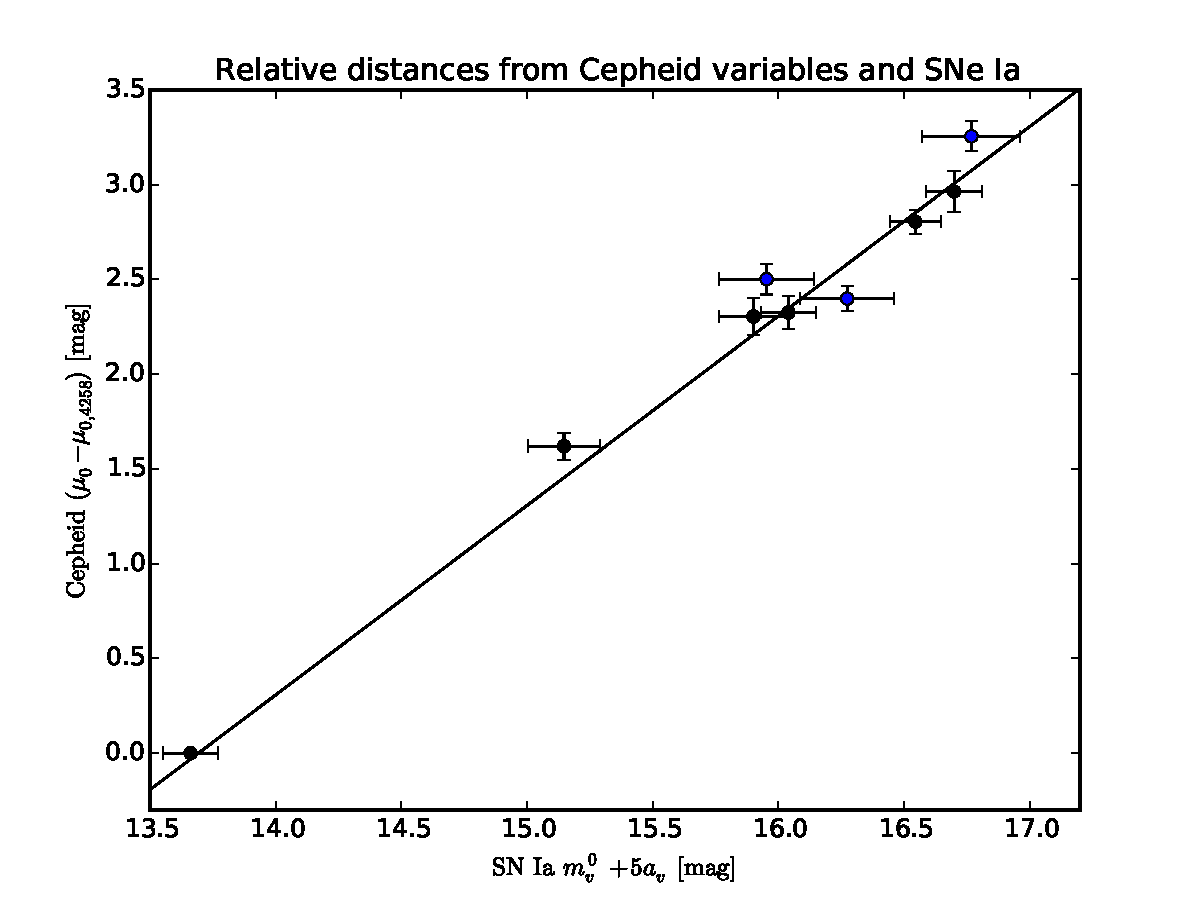
\includegraphics[scale=0.4]{../figures/chapter-h0/effective_HP_SNIa.pdf} 
\end{figure}}

\only<6>{
\begin{figure}
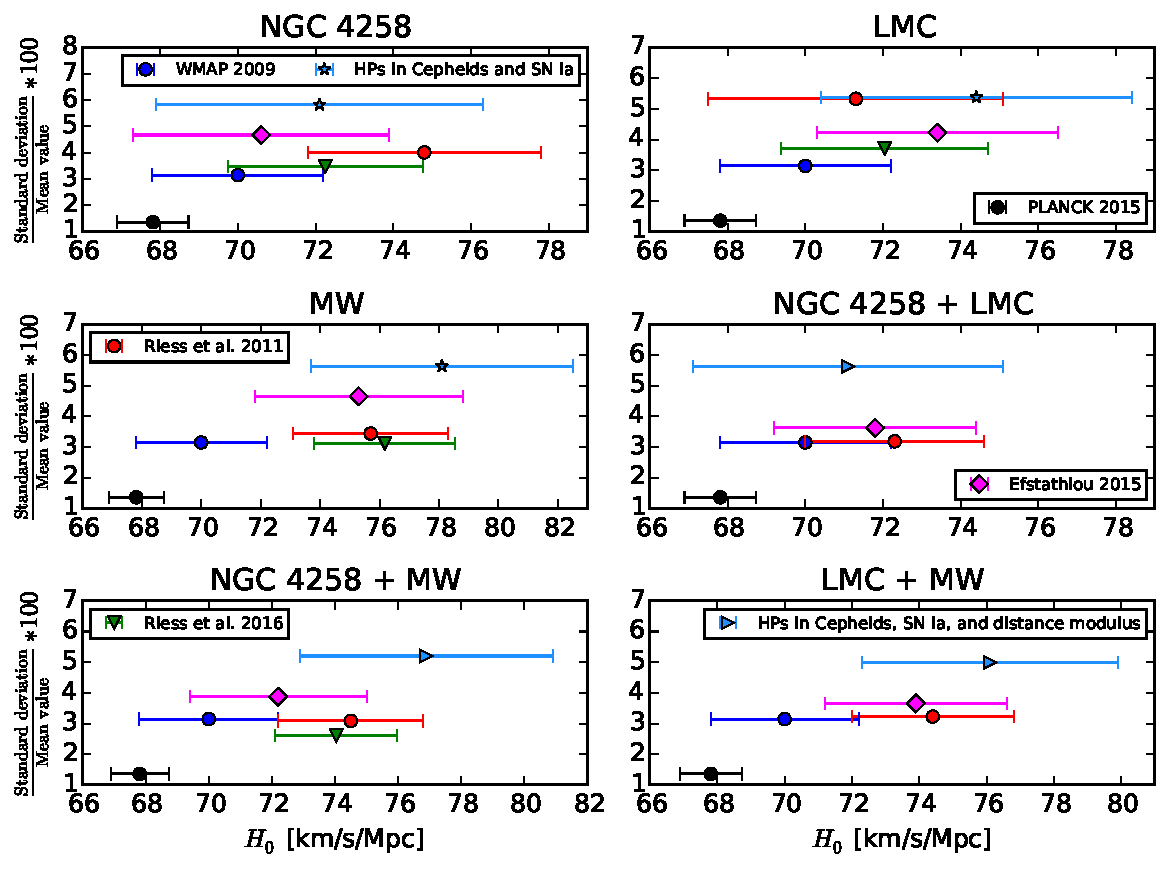
\includegraphics[scale=0.4]{../figures/chapter-h0/H0_values_anchor_combination.pdf} 
\end{figure}
}

\begin{itemize}
\only<1>{ 
\item Find no reasons to exclude data sets: period-luminosity relation compatible with direct distance determinations}
\only<2>{
\item Precision of $H_0$ depends on which data are included with HPs}
\only<3>{
\item Down-weighted fraction in Cepheid sample}
\only<4>{
\item Inconsistencies in $\SNe$ data}
\only<5>{
\item Baseline result for the R11 data set
\begin{equation*}\label{Eq:H0-value-standard-analysis}
	H_0 = 75.0 \pm 3.9 \, \mathrm{km/s/Mpc} \, 
\end{equation*}
}
\only<6>{
\item Anchor choice and comparison with previous results}
\end{itemize}
\end{frame}

\begin{frame}{Project 4: measuring the Hubble constant}{Results: the R16 data set}

\only<1-2>{
\begin{figure}
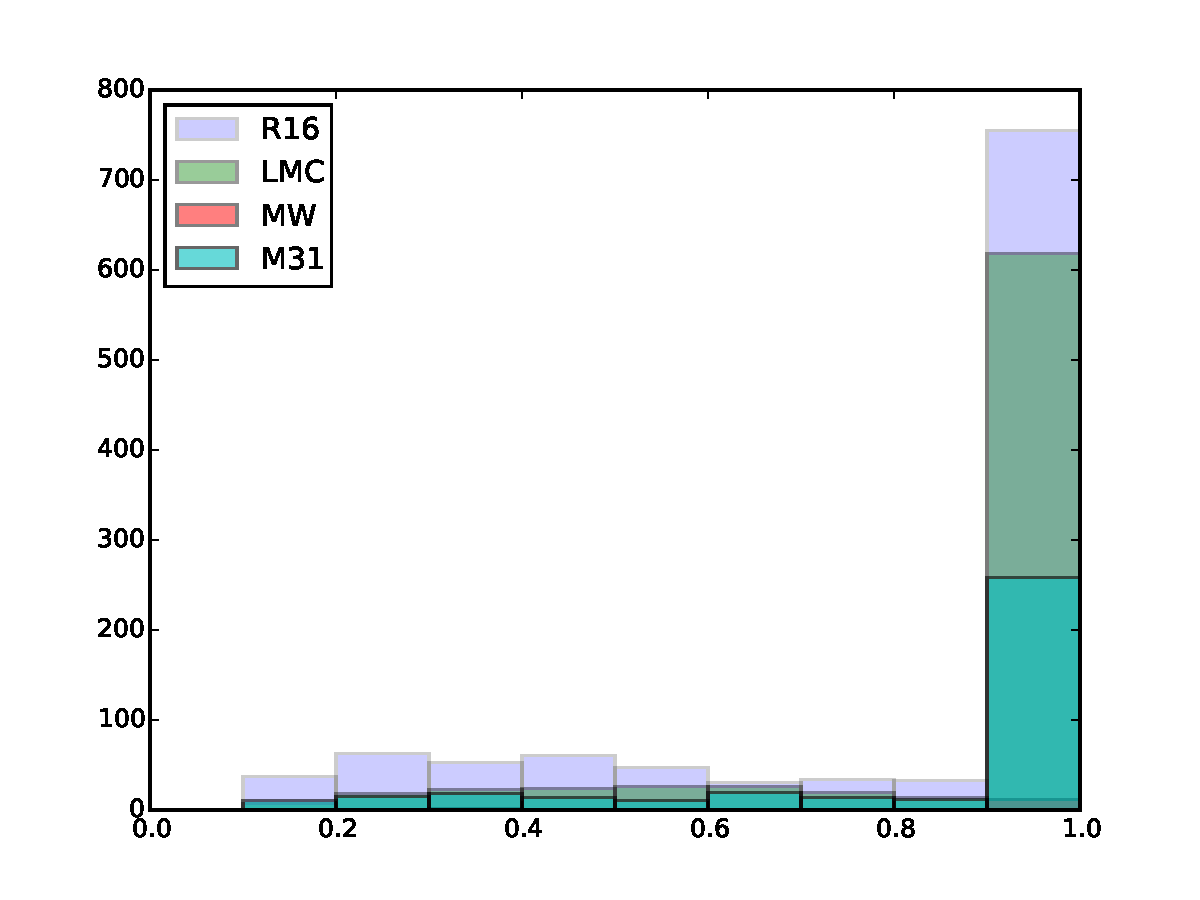
\includegraphics[scale=0.4]{../figures/chapter-h0/effective_HP_histogram_R16.pdf} 
\end{figure}}
\only<3>{
\begin{figure}
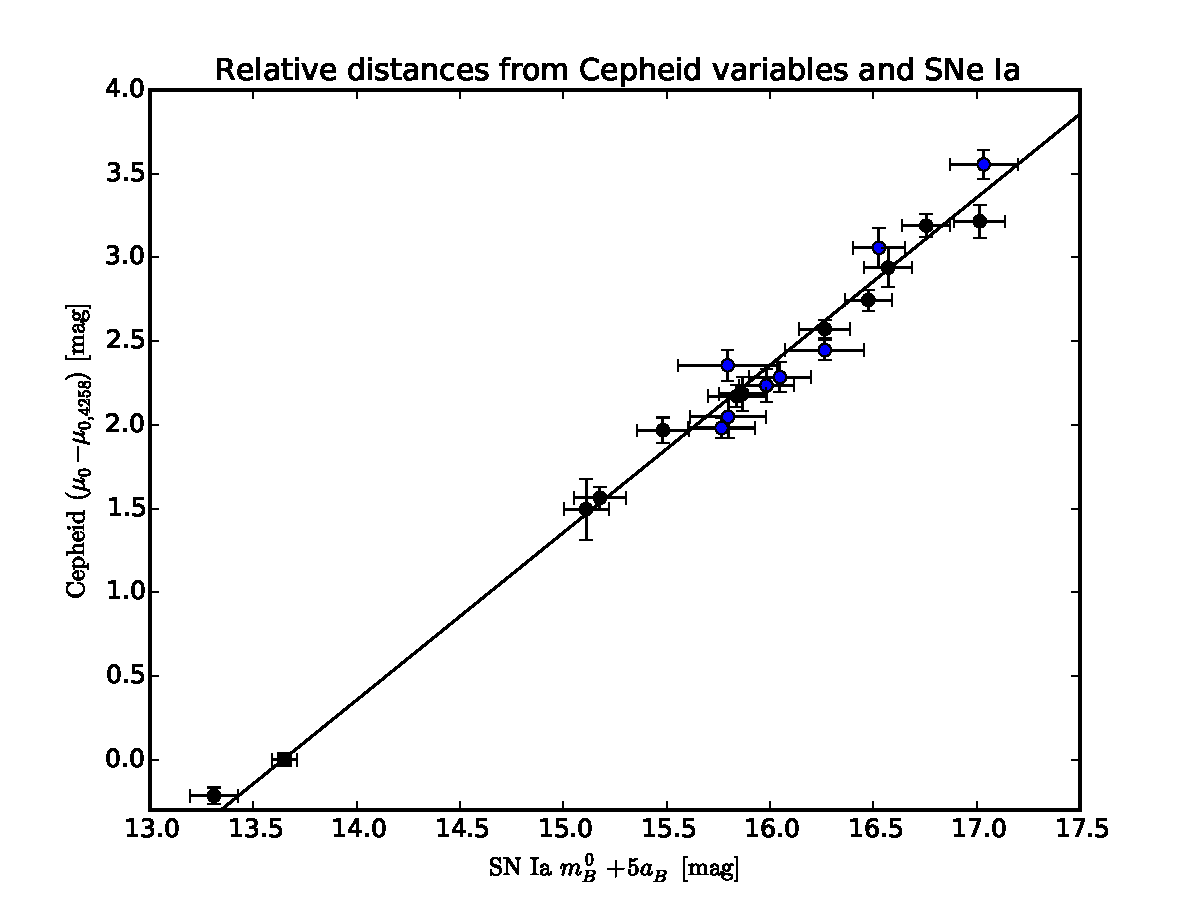
\includegraphics[scale=0.4]{../figures/chapter-h0/effective_HP_SNIa_R16.pdf} 
\end{figure}}

\only<6>{
\begin{table}[tbp]
\centering
\begin{tabular}{@{}ccccc}
\hline
\multicolumn{4}{c}{Consistency of different kinds of data} \\
\hline
Data set &$|| \alpha^{\Cepheid}||$ & $|| \alpha^{\SNe}||$ & $|| \alpha^{\Anchors}||$ \\
\hline
 R11 &  $ 0.72 $ & $ 0.74 $ & $0.86$  \\
 
 R16 &  $ 0.86 $ & $ 0.78 $ & $0.92$  \\
  
% f & $\NGC$ & $-6.12\,(0.15)$&$-3.02\,(0.17)$ & $0.12$  \\

\hline
\end{tabular}
%\caption{\label{Table:fits-section-4-1} \wct{Constraints for the parameters in the period-luminosity relation. Numbers in brackets indicate the standard deviation. Fit (c) was derived using the distance modulus in Eq. \eqref{Eq:LMC-measured-distance-modulus}, fit (e) corresponds to Eq. \eqref{Eq:MW-bestfit}, and fit (f) was derived using the distance modulus in Eq. \eqref{Eq:NGC4258-measured-distance-modulus-2013}}.}
\end{table}}

\only<7>{
\begin{figure}
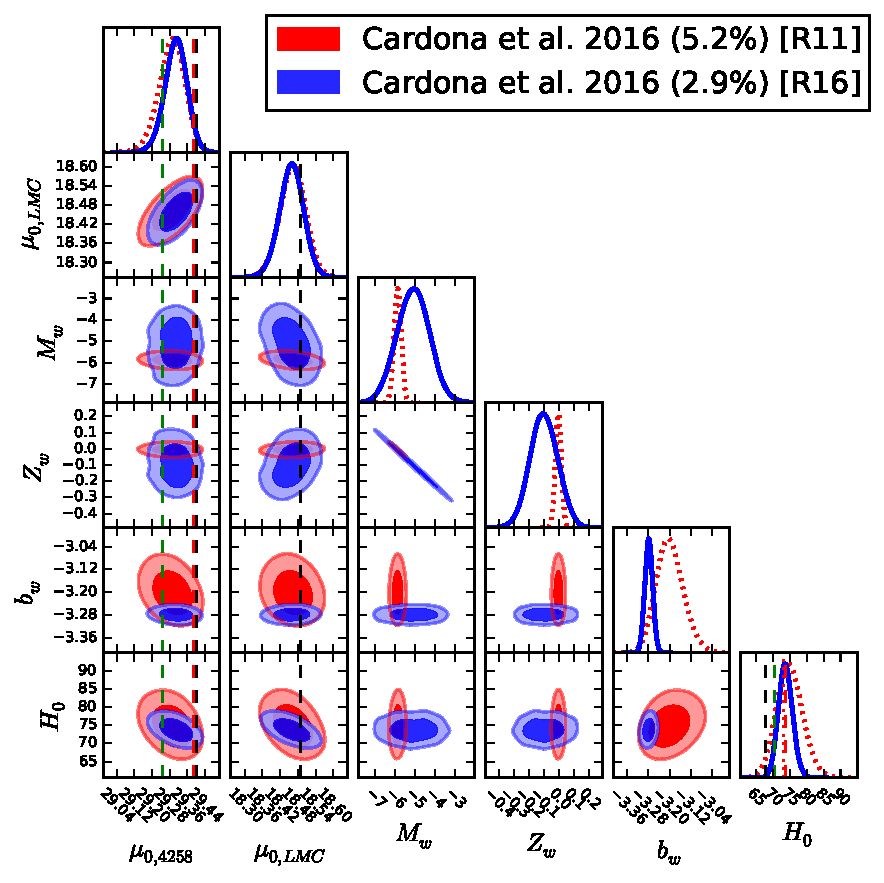
\includegraphics[scale=0.5]{../figures/chapter-h0/triangle_plot_fit_29_44.pdf} 
\end{figure}}

\only<8>{
\begin{figure}
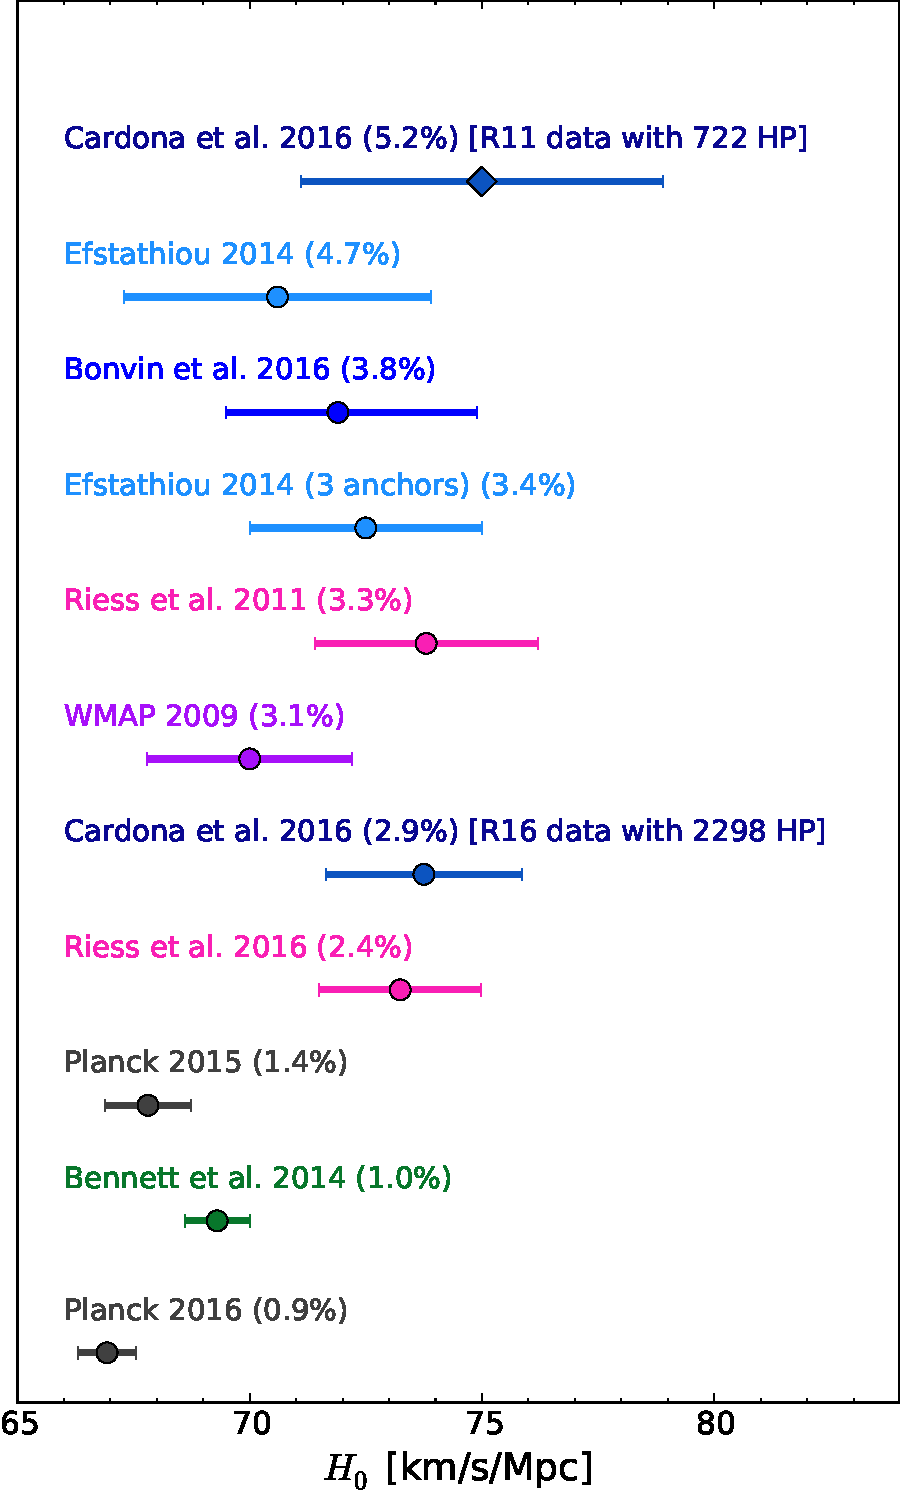
\includegraphics[scale=0.3]{../figures/chapter-h0/H0_best_estimates.pdf} 
\end{figure}}

\begin{itemize}
\only<1>{
\item No outliers released in the Cepheid sample, however...}
\only<2>{
\item Down-weighted fraction in Cepheid sample}
\only<3>{
\item Inconsistencies in $\SNe$ data}
\only<4-5>{
\item Consider variants of baseline analysis (e.g., period cut-off, metallicity dependence, reddening law) and compute systematic error due to these changes 
\begin{equation*}
\sigma_{\rm syst}=0.20 \km\, \second^{-1}\, \Mpc^{-1} 
\end{equation*}}
\only<5>{
\item Baseline result for the R11 data set
\begin{equation*}
H_0 = 73.75 \pm 2.11\,\km\, \second^{-1}\, \Mpc^{-1},
\label{Eq:primary-best-fit-R16}
\end{equation*}}
\only<6>{
\item Improvement of compatibility of different kinds of data}
\only<7>{
\item }
\only<8>{ 
\item }
\end{itemize}
\end{frame}

%\begin{frame}{Project 4: measuring the Hubble constant}{Why do we care about a local measurement of $H_0$?}
%\begin{itemize}
%\item Distance modulus 
%\begin{equation*}
%\mu_0 = m_B - M_B = 5 \log_{10} \left(\frac{d_L}{1 \mathrm{Mpc}} \right) + 25 \, . \label{eq:distmag}
%\end{equation*}
%\item Cepheid variables period-luminosity relation
%\begin{equation*}\label{Eq:P-L-equation}
%m_{X,i,j} = \mu_{0,i} + M_X + b_X (\log P_{i,j}-1) + Z_X \Delta \log[O/H]_{i,j},
%\end{equation*}
%\item SN Ia magnitudes
%\begin{equation*}
%5 \log_{10} H_0 = m_V - \mu_0 + 5a_v + 25 \, . \label{eq:h0formalism}
%\end{equation*}
%\end{itemize}
%\end{frame}

%\section{Method: Bayesian hyper-parameters (HP)}

%\begin{frame}{Method: Bayesian hyper-parameters (HP)}
%\begin{itemize}
%\item \textbf{Trust no one}. Some error bars may have been underestimated (e.g., unrecognised systematic effects), then allow for a rescaling $\sigma_i \rightarrow \sigma_i/\sqrt{\alpha_i}$.
%\item 
%\only<2>{Assume Gaussian likelihood for the data $D_i$
%\begin{equation*}
%P_G(D_i|\vec{w}) = \tilde{N}_i \, \frac{\exp(-\chi^2_i(\vec{w})/2)}{\sqrt{2\pi}},
%\end{equation*}}
%\only<3>{where  
%\begin{equation*}
%\chi^2_i \equiv \frac{\left( x_{\obs,i} - x_{\pred,i}(\vec{w}) \right)^2}{\sigma_i^2} \quad \mathrm{and} \quad \tilde{N}_i = \frac{1}{\sqrt{\sigma_i^2}}. 
%\end{equation*}}
%\only<4>{Control relative weight of data points in the likelihood with HP $\alpha_i$, likelihood becomes
%\begin{equation*}
%P(D_i|\vec{w},\alpha_i) = \tilde{N}_i \, \alpha_i^{1/2}\, \frac{\exp(-\alpha_i \chi^2_i(\vec{w})/2)}{\sqrt{2\pi}}.
%\end{equation*}}
%\only<5>{For a given model with parameters $\vec{w}$ and a set of $N$ data points $ \lbrace D_i \rbrace$ 
%\begin{equation*}
%P(\vec{w}|\lbrace D_i \rbrace) = \int \dots \int P(\vec{w},\lbrace \alpha_i \rbrace|\lbrace D_i \rbrace)\, d\alpha_1 \dots d\alpha_N,
%\end{equation*}}
%\only<6>{From Bayes' theorem
%\begin{equation*}
%P(\vec{w},\lbrace \alpha_i \rbrace|\lbrace D_i \rbrace) = \frac{P(\lbrace D_i \rbrace|\vec{w},\lbrace \alpha_i \rbrace)\, P(\vec{w},\lbrace \alpha_i \rbrace)}{P(D_1,\dots,D_N)},
%\end{equation*}
%\begin{equation*}
%P(\vec{w},\lbrace \alpha_i \rbrace) = P(\vec{w}|\lbrace \alpha_i \rbrace)\, P(\lbrace \alpha_i \rbrace),
%\end{equation*}
%\begin{equation*}
%P(\lbrace D_i \rbrace|\vec{w},\lbrace \alpha_i \rbrace)  = P(D_1|\vec{w},\alpha_1)\dots P(D_N|\vec{w},\alpha_N),
%\end{equation*}
%\begin{equation*}
%P(\vec{w}|\lbrace \alpha_i\rbrace)  = \mathrm{constant}
%\end{equation*}
%\begin{equation*}
%P(\lbrace \alpha_i \rbrace) = P(\alpha_1)\dots P(\alpha_N)
%\end{equation*}
%}
%\only<7>{Further assuming uniform prior for HP ($P(\alpha_i)=1$) and that errors are never smaller than their reported value ($\alpha_i \in [0,1]$)
%\begin{equation*}
%P(\vec{w},\lbrace D_i \rbrace) = \frac{P(D_1|\vec{w})\dots P(D_N|\vec{w})}{P(D_1,\dots,D_N)},
%\end{equation*}
%\begin{equation*}
%P(D_i|\vec{w}) \equiv \int_0^1 P(D_i|\vec{w},\alpha_i)\, d\alpha_i.
%\end{equation*}
%}
%\only<8>{In the case of a Gaussian HP likelihood
%\begin{equation*}
%P(D_i|\vec{w}\,) = \tilde{N}_i \, \left(\frac{ \mathrm{Erf}\left( \frac{\chi_i(\vec{w})}{\sqrt{2}} \right)  -\sqrt{\frac{2}\pi} \chi_i(\vec{w}) \exp(-\chi^2_i(\vec{w})/2)}{ \chi^3_i(\vec{w})} \right)
%\end{equation*}
%}
%\only<9>{Rewriting
%\begin{equation*}
%\ln P(\vec{w},\lbrace D_i \rbrace) = \sum_i \ln \tilde{N}_i + \ln \tilde{\chi}^2_i
%\end{equation*}
%\begin{equation*}
%\tilde{\chi}^2_i(\chi^2_i(\vec{w})) \equiv \frac{ \mathrm{Erf}\left( \frac{\chi_i(\vec{w})}{\sqrt{2}} \right)  -\sqrt{\frac{2}\pi} \chi_i(\vec{w}) \exp(-\chi^2_i(\vec{w})/2)}{ \chi^3_i(\vec{w})}
%\end{equation*}
%}
%\only<10>{Effective HP for each data point are given by
%\begin{eqnarray*}
%\alpha^{\eff}_i & = 1,\quad \mathrm{if} \quad \chi^2_i\leq1
%\\
%\label{Eq:effective-HP-2}
%\alpha^{\eff}_i & = \frac{1}{\chi^2_i},\quad \mathrm{if} \quad \chi^2_i> 1.
%\end{eqnarray*}
%}
%\end{itemize}
%
%\end{frame}

%\section{Applying HP: Period-Luminosity relation}

%\begin{frame}{Applying HP: Cepheid variables}{P-L relation}
%Period luminosity relation, distance modulus, apparent magnitude for SN Ia
%\includegraphics[scale=0.4]{../../../../../projects/B/cmb-maps/planck-nside/gaussian/map_2000.pdf} 
%\end{frame}

%\begin{frame}{Applying HP}{Large Magellanic Cloud (LMC)}
% 
% 
%\only<1>{LMC figure}%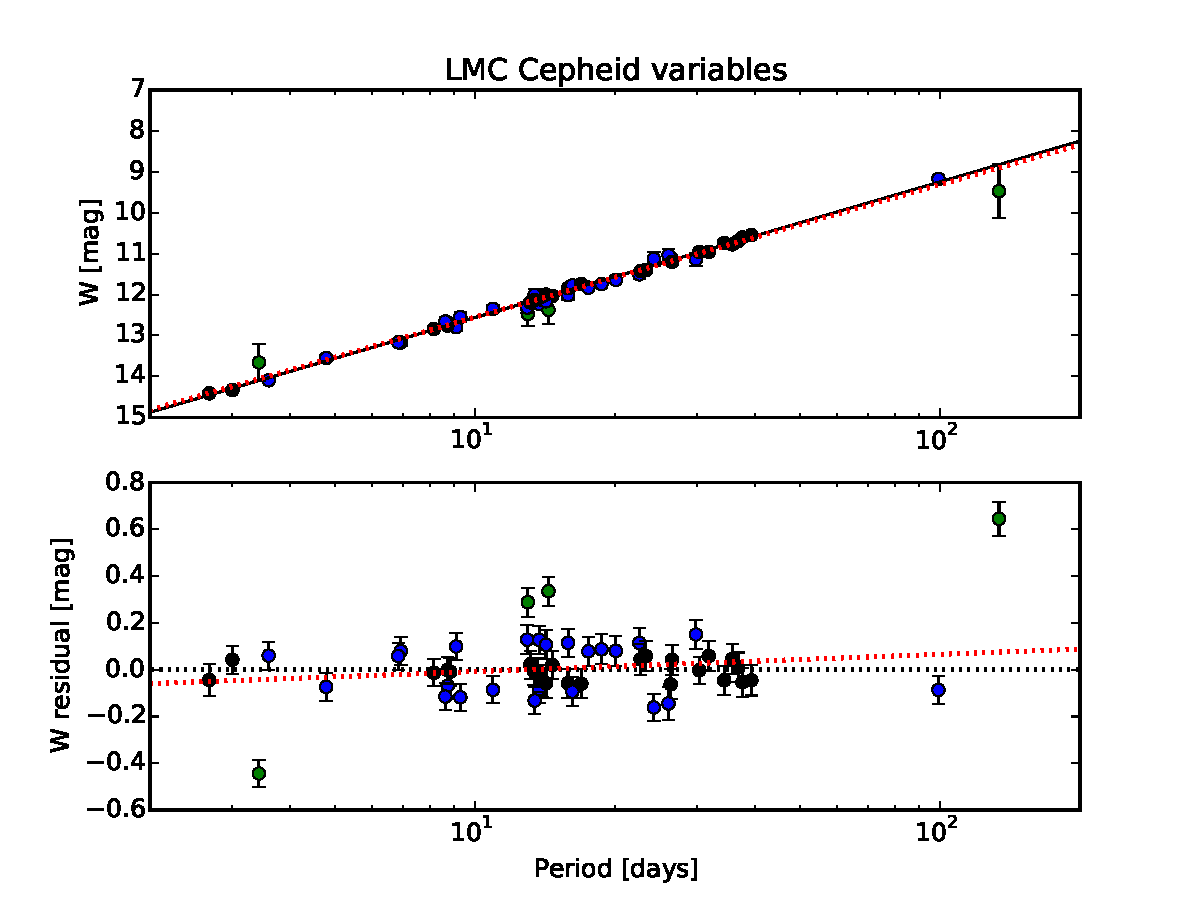
\includegraphics[scale=0.5]{../Draft/effective_HP_cepheids_LMC.pdf} }
%\only<2>{
%\begin{table}[tbp]
%\centering
%\begin{tabular}{@{}ccccc}
%\hline
%\multicolumn{5}{c}{LMC Cepheid variables} \\
%\hline
%Fit & $A$ & $b_W$ & $\sigma_{\intt}^{\LMC}$ & Period cut \\
%\hline
% a & $12.570\,(0.035)$ & $-3.32\,(0.10)$ & $0.06$ & $10<P<60$ \\
%  
% b & $12.562\,(0.016)$&$-3.30\,(0.05)$ & $0.06$ & $P<60$ \\
%
% c & $12.562\,(0.016)$& $-3.31\,(0.05)$& $0.06$ & $P<205$ \\
%
% d & $12.555\,(0.019)$& $-3.24\,(0.06)$& $0.12$ & $P<205$ \\
%\hline
%\end{tabular}
%\end{table}
%
%\begin{equation*}
%\mu_{0,\LMC}^{\rm M} = 18.49 \pm 0.05, \quad M_W = -5.93 \pm 0.07
%\end{equation*}
%}
%\end{frame}

%\begin{frame}{Applying HP}{Milky Way (MW)}
%\centering
%MW figure
%%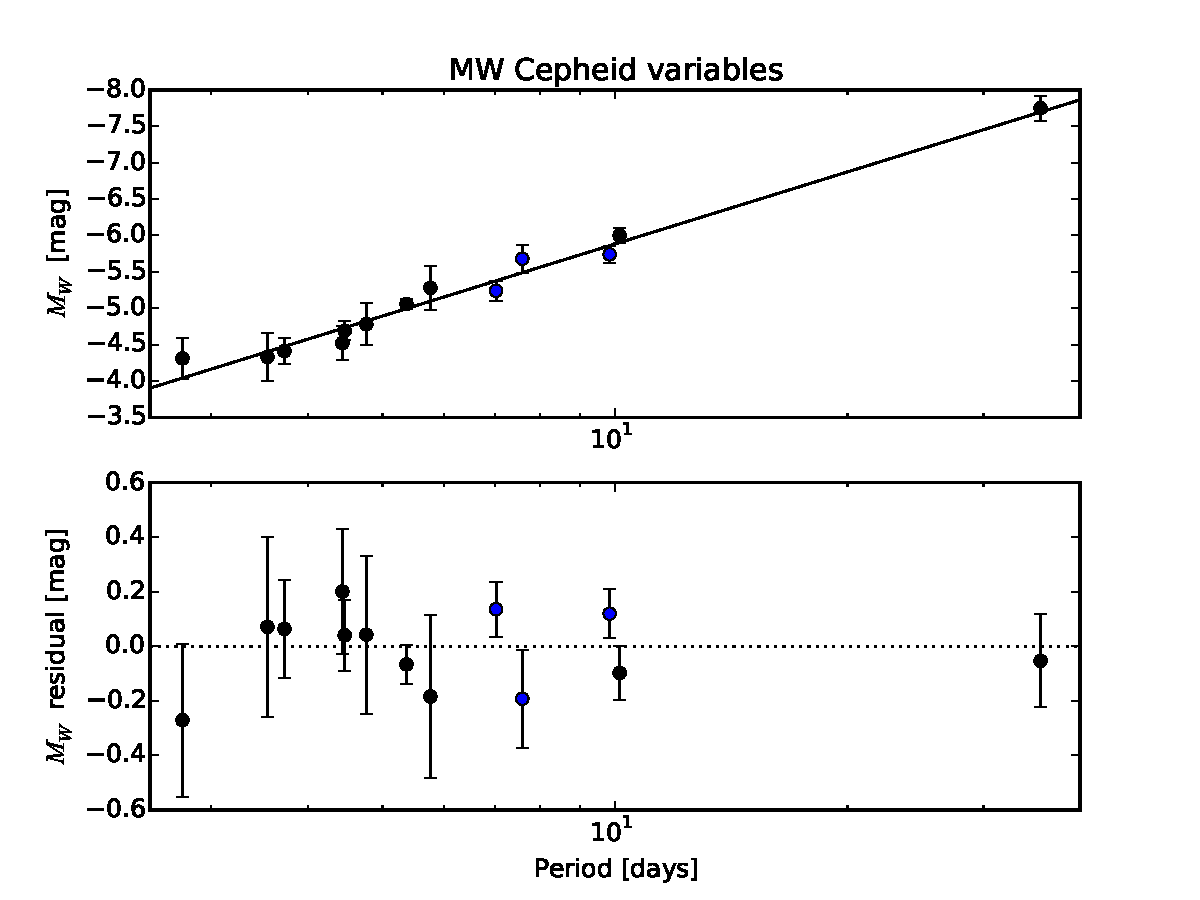
\includegraphics[scale=0.45]{../Draft/effective_HP_cepheids_MW.pdf}
%\begin{equation*}\label{Eq:MW-bestfit}
%M_W = -5.88 \pm 0.07  , \qquad b_W = -3.30 \pm 0.26  , \qquad \sigma_{\intt}^{\MW} = 0.02 ,
%\end{equation*}
%\end{frame}

%\begin{frame}{Applying HP}{Megamaser system NGC 4258}
%\only<1>{4258 figure%\centering
%%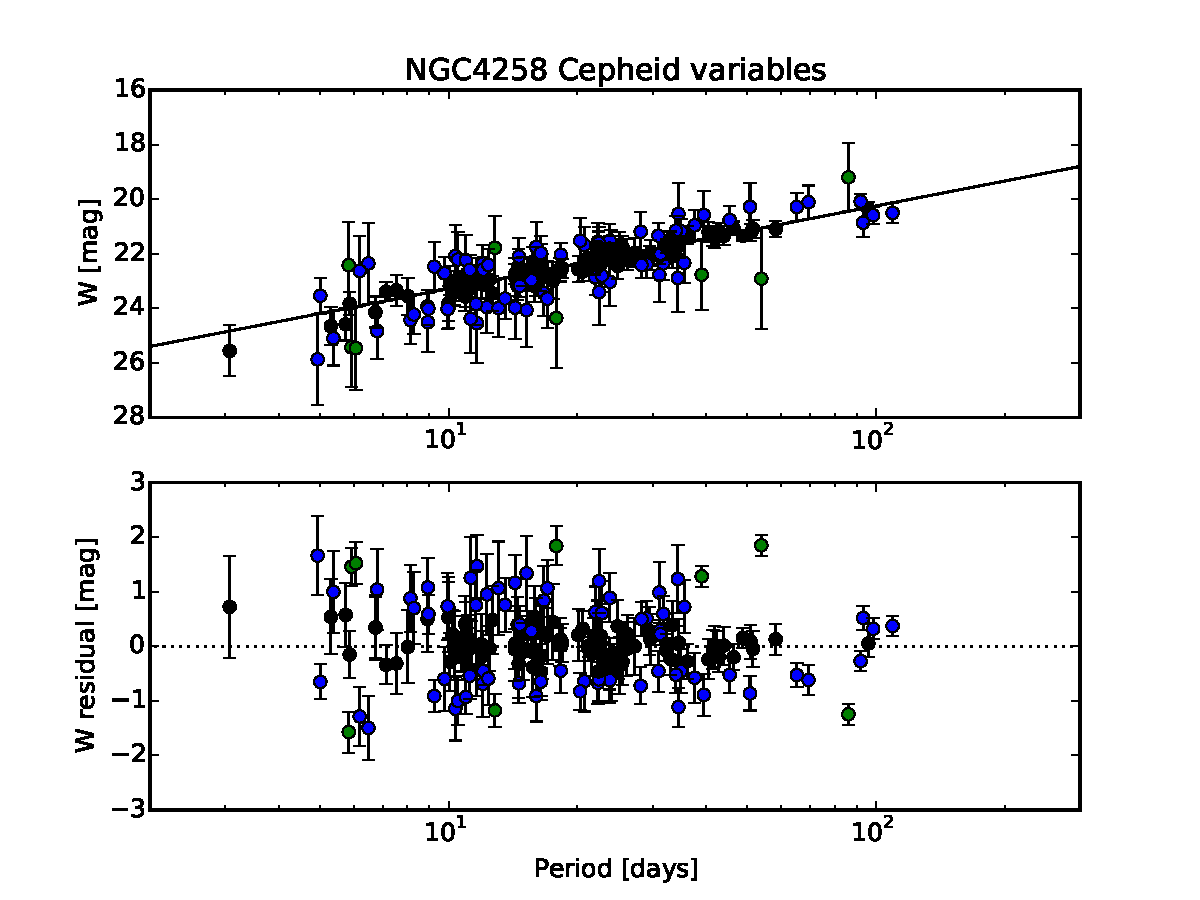
\includegraphics[scale=0.45]{../Draft/effective_HP_cepheids_NGC4258.pdf}
%\begin{equation*}
%\mu_{0,\rm 4258} = 29.40 \pm 0.07, \qquad M_W=-6.12 \pm 0.15, \quad b_W = -3.02 \pm 0.17  , \qquad \sigma_{\intt}^{\rm NGC4258} = 0.12 .
%\end{equation*} }
%\only<2>{\centering
%I do not see any reason to discard those data sets }
%\end{frame}

%\section{The Hubble constant $H_0$}

%\begin{frame}{The Hubble constant $H_0$}{Data}
%\begin{itemize}
%\item 8 SN Ia hosts: apparent magnitudes
%\item MW Cepheid variables (parallax measurements): period, metallicity, magnitudes
%\item LMC Cepheid variables: period, metallicity, magnitudes
%\item Distance modulus to LMC derived from eclipsing binaries
%\item Distance modulus to NGC 4258 derived from geometric maser distance and from standardised candle method for type IIP SNe   
%\end{itemize}  
%%\begin{columns}
%%\begin{column}{0.45\textwidth}
%%\centering
%%\only<1-4>{Gaussian, isotropic simulation
%%\includegraphics[scale=0.2]{../../../../../projects/B/ksv-maps/planck-nside/gaussian/192c/vmap_2000.pdf}} 
%%\end{column}
%%\begin{column}{0.45\textwidth}
%%\centering 
%%\only<2-3>{Inpainted SMICA 
%%\includegraphics[scale=0.2]{../../../../../projects/B/ksv-maps/planck-nside/smica/192c/inpainted/vmap.pdf}}
%%\only<4>{Inpainted NILC 
%%\includegraphics[scale=0.2]{../../../../../projects/B/ksv-maps/planck-nside/nilc/192c/inpainted/vmap.pdf}}
%%\end{column}
%%\end{columns}
%\end{frame}

%\begin{frame}{The Hubble constant $H_0$}{The likelihood}
%\begin{itemize}
%\item Full likelihood 
%\begin{equation*}
%\ln P(\vec{w},\lbrace D_i \rbrace) = \ln P^{\Cepheid} + \ln P^{\SNe} + \ln P^{\Anchors}. 
%\end{equation*}
%\item For instance
%\begin{equation*}
%\ln P^{\Cepheid} = \sum_{ij} \ln \tilde{\chi}^{2}(\chi^{2,\Cepheid}_{ij}) + \ln \tilde{N}^{\Cepheid}_{ij},
%\end{equation*}
%\item $\SNe$, $\Anchors$,...
%%\begin{equation*}
%% \ln P^{\SNe} = \sum_{i} \ln \tilde{\chi}^{2}(\chi^{2,\SNe}_{i}) + \ln \tilde{N}^{\SNe}_{i} - \frac{(a^{R11}_v - a_v)^2}{2 \sigma_{a_v}^2} - \frac{\ln (2\pi\sigma_{a_v}^2)}{2} - \frac{(a_{\rm cal})^2}{2 \sigma_{a_{\rm cal}}^2} - \frac{\ln (2\pi\sigma_{a_{\rm cal}}^2)}{2}
%%\end{equation*}
%\end{itemize}
%%\begin{columns}
%%\begin{column}{0.45\textwidth}
%%\centering
%%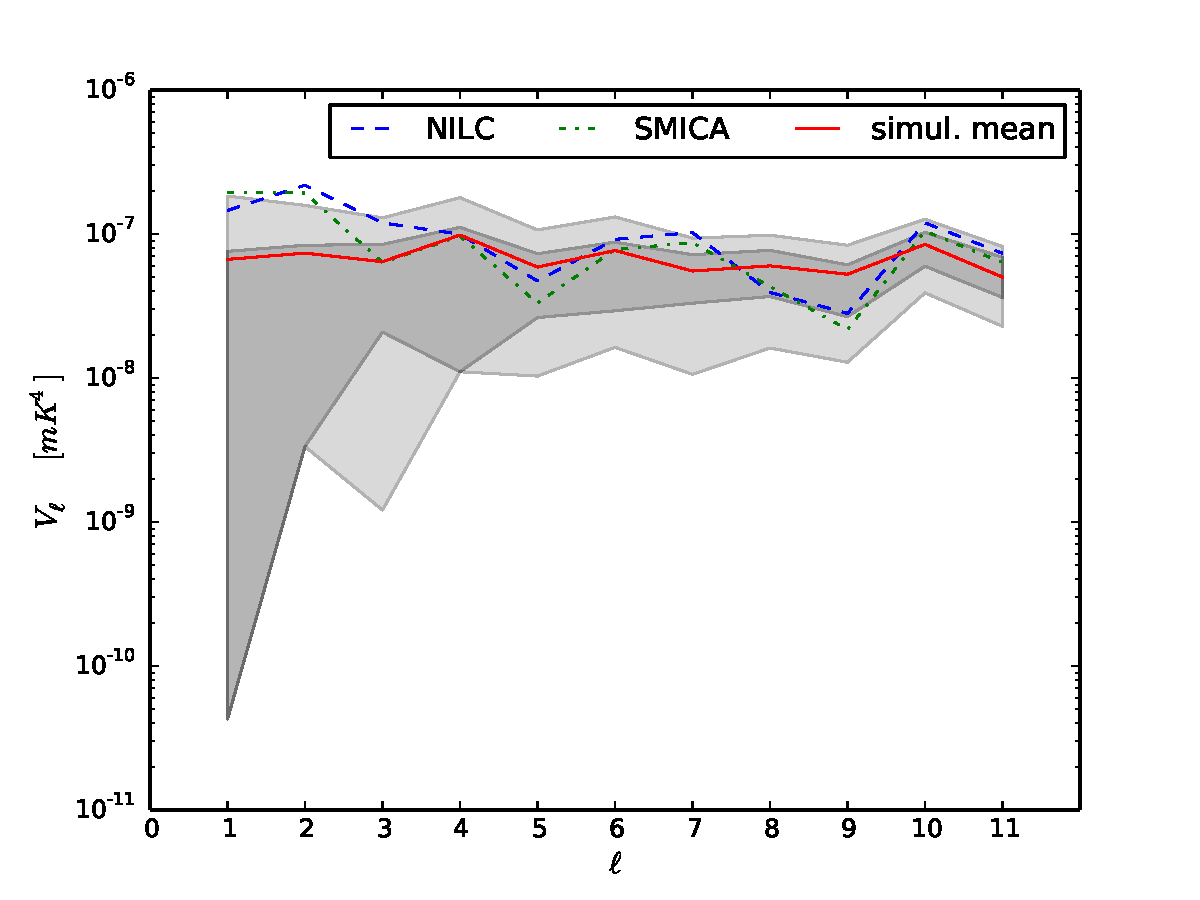
\includegraphics[scale=0.3]{../../../../../projects/B/ksv-spectra/planck-nside/plots/inpainted/192c/Inp_Vl.pdf} 
%%\end{column}
%%\begin{column}{0.45\textwidth}
%%\centering 
%%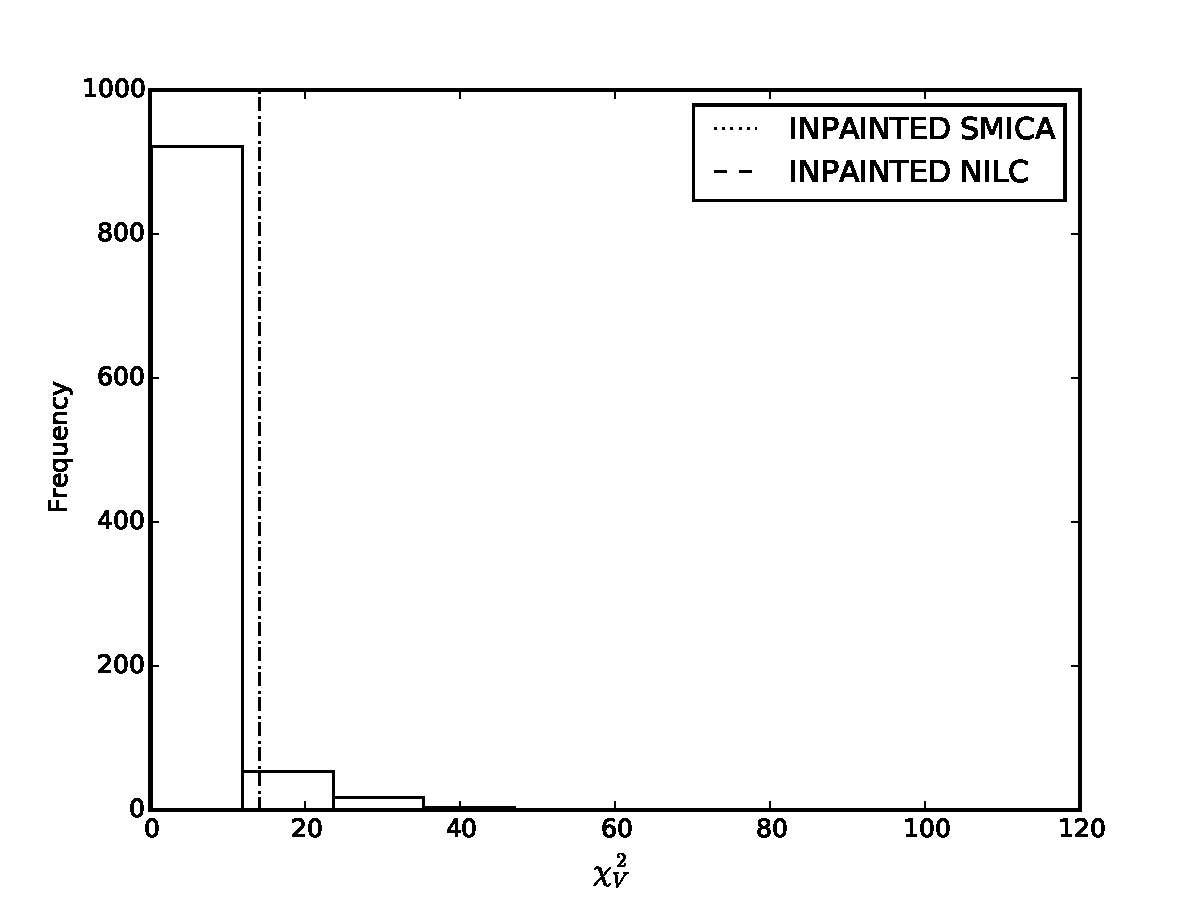
\includegraphics[scale=0.3]{../../../../../projects/B/ksv-spectra/planck-nside/plots/inpainted/192c/vchi2.pdf} 
%%\end{column}
%%\end{columns}
%\end{frame}

%\begin{frame}{The Hubble constant $H_0$}{Results}
%\begin{table}[tbp]
%\centering
%\begin{tabular}{@{}lcccccr}
%\hline
%\multicolumn{7}{c}{NGC $4258 +$ LMC $+$ MW anchors} \\
%\hline
%Fit & $H_0$ & $M_W$ & $b_W$ & $Z_W$ &$\sigma_{\intt}^{\LMC}$ & $\sigma_{\intt}^{\MW}$\\
%\hline
%$M1^{a}$ & $75.0\,(3.9)$ & $-5.87\,(0.18)$ & $-3.20\,(0.05)\,[N]$ & $-0.005\,(0.020)\,[S]$ & $0.06$& $0.02$ \\
%$M1^{af}$ & $74.9\,(3.9)$ & $-5.88\,(0.18)$ & $-3.20\,(0.05)\,[N]$ & $-0.005\,(0.020)\,[S]$ & $0.06$& $0.02$ \\
%$M1^{ag}$ & $73.3\,(2.4)$ & $-5.88\,(0.18)$ & $-3.19\,(0.05)\,[N]$ & $-0.004\,(0.020)\,[S]$ & $0.06$& $0.02$ \\
%$M1^{ah}$ & $74.6\,(1.9)$ & $-5.89\,(0.17)$ & $-3.21\,(0.05)\,[N]$ & $-0.005\,(0.020)\,[S]$ & $0.06$& $0.02$ \\
%$M1^{aj}$ & $72.4\,(2.2)$ & $-5.90\,(0.18)$ & $-3.20\,(0.05)\,[N]$ & $-0.004\,(0.020)\,[S]$ & $0.06$& $0.02$ \\
%$M1^{b}$ & $76.1\,(3.1)$ & $-5.86\,(0.17)$ & $-3.27\,(0.04)\,[N]$ & $-0.007\,(0.019)\,[S]$ & $0.06$ & $0.02$ \\
%$M1^{be}$ & $75.1\,(3.4)$ & $-5.89\,(0.18)$ & $-3.25\,(0.07)\,[N]$ & $-0.004\,(0.020)\,[S]$ & $0.113$ & $0.10$ \\
%$M2^{a}$ & $74.7\,(4.0)$ & $-4.68\,(0.97)$ & $-3.20\,(0.05)\,[N] $ & $-0.141\,(0.110)\,[W] $ & $0.06 $ & $0.02 $ \\
%$M2^{b}$ & $ 75.1\,(3.8)$ & $-3.84\,(1.05)$ & $-3.28\,(0.04)\,[N]$ & $-0.236\,(0.119)\,[W]$ & $0.06$ & $0.02$ \\
%$M3^{a}$ & $75.0\,(3.9)$ & $-5.92\,(0.04)$ & $-3.20\,(0.05)\,[N]$ & $0$ & $0.06$ & $0.02$ \\
%$M3^{b}$ & $75.4\,(3.7)$ & $-5.92\,(0.04)$ & $-3.27\,(0.04)\,[N]$ & $ 0 $ & $0.06$ & $0.02$ \\
%$M4^{a}$ & $74.7\,(4.0)$ & $-4.35\,(1.11)$ & $-3.20\,(0.05)\,[N]$ & $-0.178\,(0.125)\,[N]$ & $0.06$ & $0.02$ \\
%$M4^{b}$ & $75.2\,(3.9)$ & $-3.18\,(1.25)$ & $-3.28\,(0.04)\,[N]$ & $-0.311\,(0.141)\,[N]$ & $0.06$ & $0.02$ \\
%\hline
%
%\end{tabular}
%
%\end{table}
%%\begin{columns}
%%\begin{column}{0.45\textwidth}
%%\centering
%%\only<1-4>{Gaussian, isotropic simulation
%%\includegraphics[scale=0.2]{../../../../../projects/B/ksv-maps/planck-nside/gaussian/192c/smap_2000.pdf}} 
%%\end{column}
%%\begin{column}{0.45\textwidth}
%%\centering 
%%\only<2-3>{Inpainted SMICA 
%%\includegraphics[scale=0.2]{../../../../../projects/B/ksv-maps/planck-nside/smica/192c/inpainted/smap.pdf}}
%%\only<4>{Inpainted NILC 
%%\includegraphics[scale=0.2]{../../../../../projects/B/ksv-maps/planck-nside/nilc/192c/inpainted/smap.pdf}}
%%\end{column}
%%\end{columns}
%\end{frame}

%\begin{frame}{The Hubble constant $H_0$}{Results: fit $M1^a$}
%
%%\begin{columns}
%%\begin{column}{0.45\textwidth}
%\begin{figure}
%Triangle plot
%%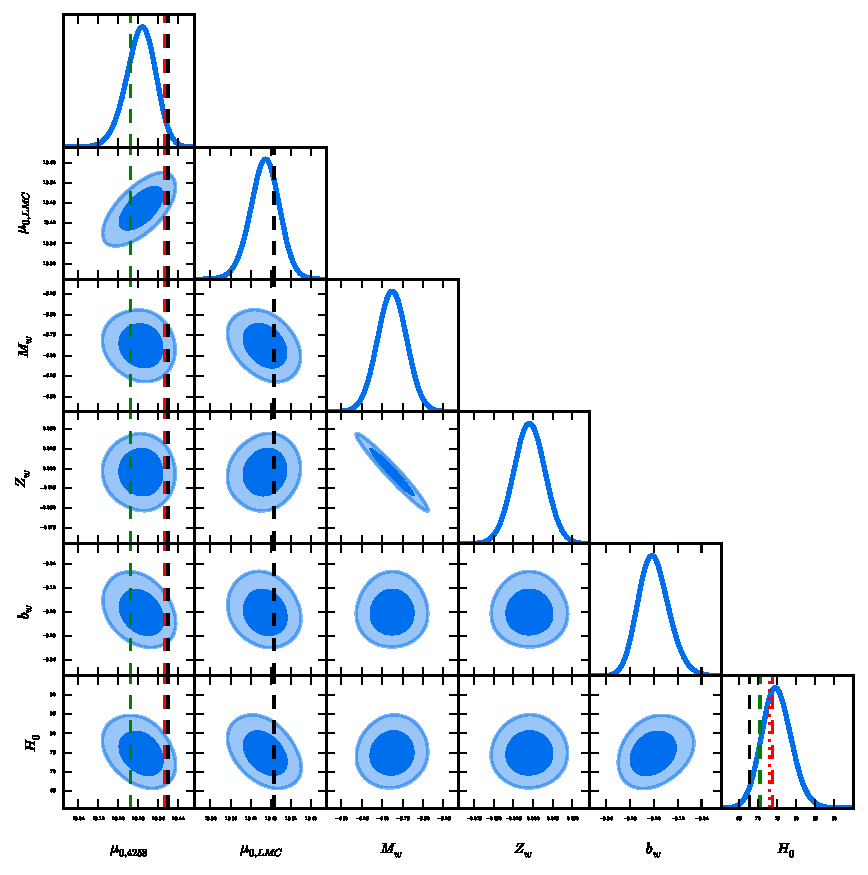
\includegraphics[scale=0.5]{../Draft/triangle_plot.pdf} 
%\end{figure}
%
%%\end{column}
%%\begin{column}{0.45\textwidth}
%%\centering 
%%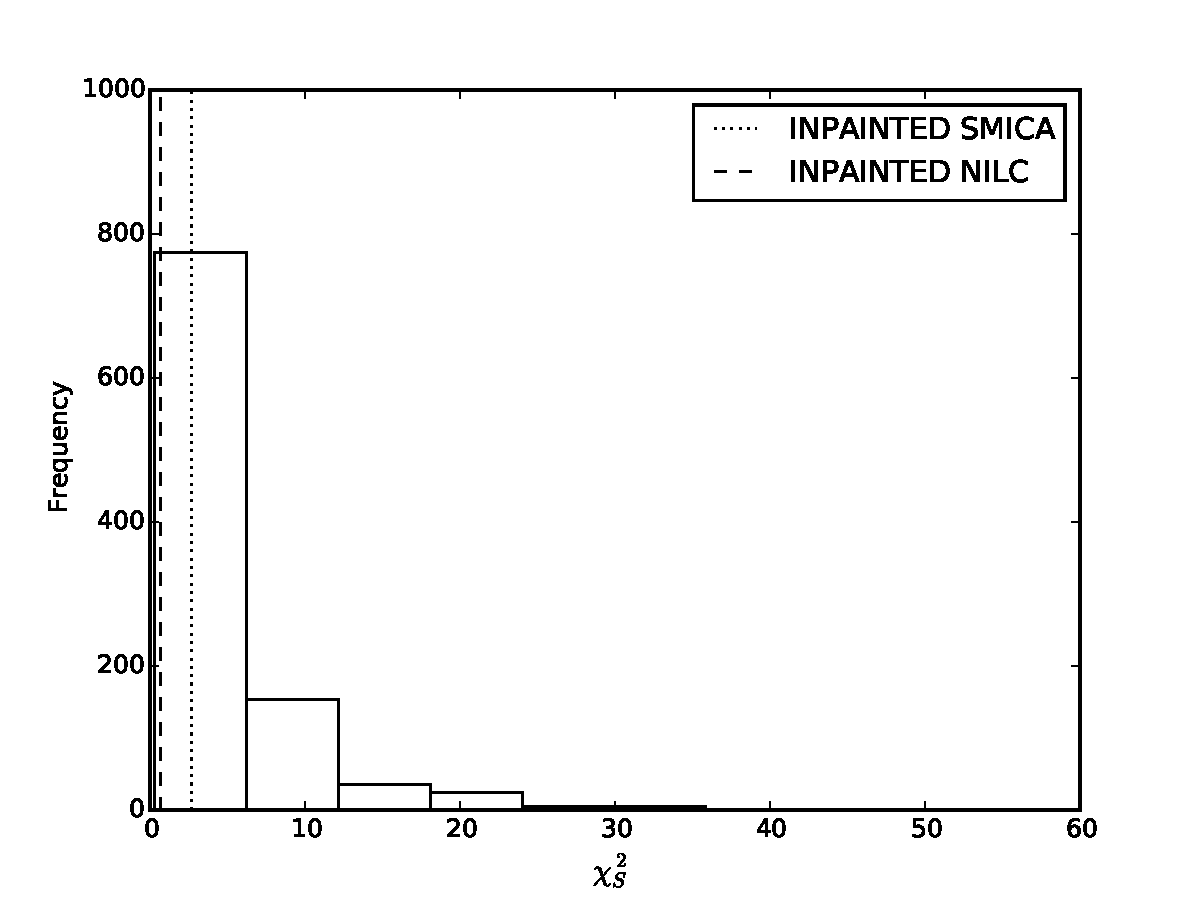
\includegraphics[scale=0.3]{../../../../../projects/B/ksv-spectra/planck-nside/plots/inpainted/192c/schi2.pdf} 
%%\end{column}
%%\end{columns}
%\end{frame}

%\begin{frame}{The Hubble constant $H_0$}{Conclusions}
%\begin{itemize}
%\item If one trust no one (HPs everywhere) $H_0=75.0\pm3.9$ a $5\%$ measurement.
%\item Trust only distance modulus (no HPs) $H_0=74.6\pm1.9$  ($2.5\%$)
%\item Trust only SN Ia $H_0=73.3\pm2.4$ ($3.3\%$)
%\item Distrust both SN Ia and distance modulus data $H_0=72.4\pm2.2$  ($3\%$) 
%\item Anchors choice: no reason to discard data
%\item Metallicity: cannot say much about this with available data
%\item Period cut: does not matter in our method
%\item Results agree with R16: 18 SN Ia hosts, better distance modulus to NGC4258, consistent values of $H_0$, no outlier rejection needed any longer (they claim), no outliers among SN Ia hosts
%%\item Do not reject data, keep the data and study the physics! (Adam Riess)
%\end{itemize}
%\end{frame}

%\begin{frame}{The Hubble constant $H_0$}{Conclusions}
%H0 valuess
%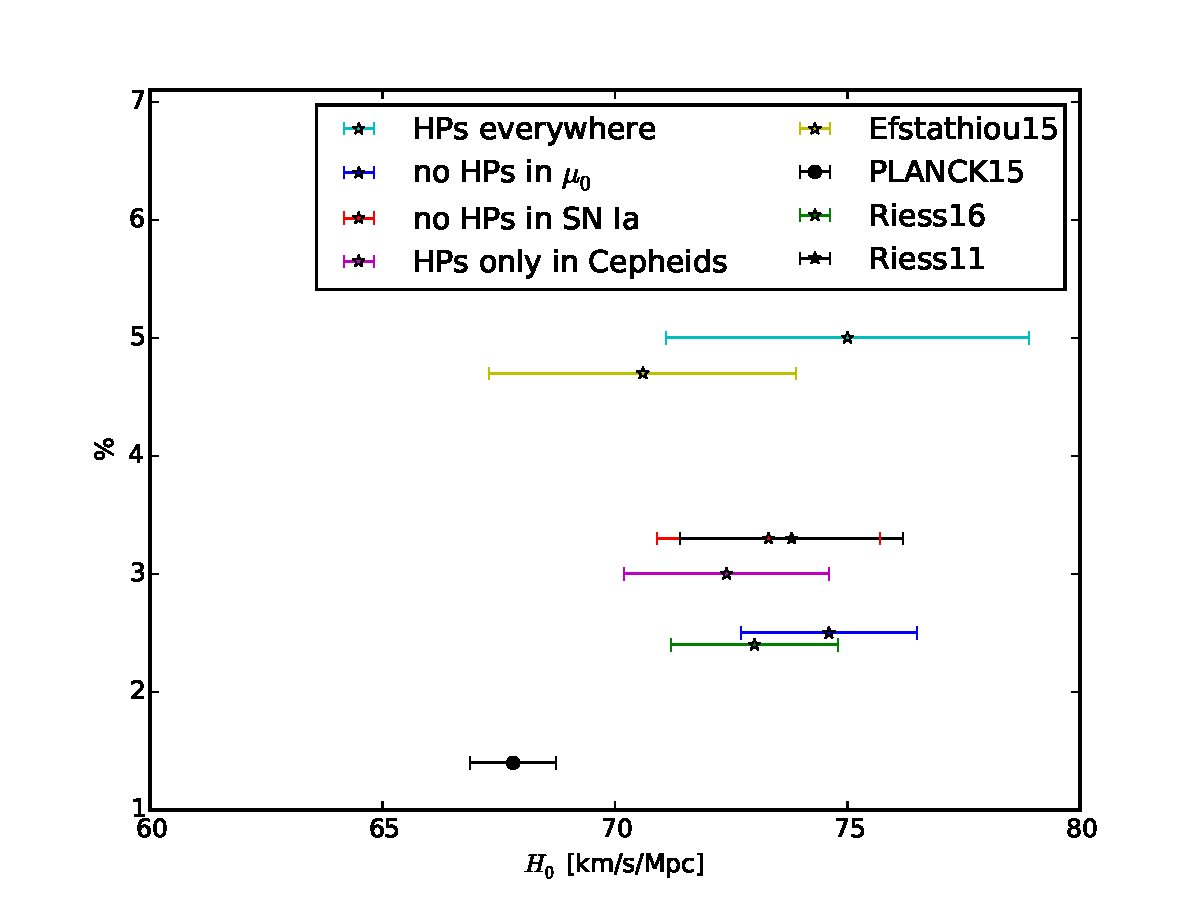
\includegraphics[scale=0.5]{./H0_values_2.pdf} 
%\end{frame}
%\begin{columns}
%\begin{column}{0.45\textwidth}
%\centering
%\only<1-4>{Gaussian, isotropic simulation
%\includegraphics[scale=0.2]{../../../../../projects/B/ksv-maps/planck-nside/gaussian/192c/kmap_2000.pdf}} 
%\end{column}
%\begin{column}{0.45\textwidth}
%\centering 
%\only<2-3>{Inpainted SMICA 
%\includegraphics[scale=0.2]{../../../../../projects/B/ksv-maps/planck-nside/smica/192c/inpainted/kmap.pdf}}
%\only<4>{Inpainted NILC 
%\includegraphics[scale=0.2]{../../../../../projects/B/ksv-maps/planck-nside/nilc/192c/inpainted/kmap.pdf}}
%\end{column}
%\end{columns}
%\end{frame}

\section{Conclusions}

\begin{frame}{Conclusions}
\begin{itemize}
\item Developed a method to search for deviations of statistical isotropy: CMB data from Planck is consistent with the Cosmological principle. 
\item Data is consistent with zero dark energy anisotropic stress
\item Lensing convergence must be included in analyses of upcoming galaxy surveys
\item Developed a method to measure the Hubble constant and asses consistency of data sets. Confirmed tension CMB and local measurements might suggest new physics or unaccounted systematics in CMB data    
\end{itemize}
\end{frame}

\end{document}



